% ----------------------------------------------------------------------
%
%                         Computer Science VII
%
%                   http://ls7-www.cs.uni-dortmund.de
%
%   questions and representations: info@ls7.cs.uni-dortmund.de
%
%   status: 20.12.2017
%
% ----------------------------------------------------------------------

\RequirePackage{ifthen}
\newcommand \Thesistyp{Masterarbeit}
\newcommand \Author{Jessica Buehler}
\newcommand \Thesistitle{Zeit-effizientes Training von Convolutional Neural Networks}
\newcommand \FirstSupervisor{Prof.~Dr.~Heinrich~M\"uller}
\newcommand \SecondSupervisor{M.Sc.~Matthias~Fey}
\newcommand \FirstChair{Lehrstuhl VII}
\newcommand \FirstChairTitle{Informatik}


% -----------------------------------------------------------------------------------------
% Option: Zweiter Lehrstuhl
\newboolean{boolNoSecondChair}
\setboolean{boolNoSecondChair}{true} % boolNoSecondChair==false: second chair involved
\ifthenelse{\boolean{boolNoSecondChair}}{
\newcommand \SecondChair{}
\newcommand \SecondChairTitle{}
}{
\newcommand \SecondChair{Computer Science XII}
\newcommand \SecondChairTitle{Embedded Systems}
}

\RequirePackage{ifpdf} \ifpdf
  \pdfoutput=1
  \pdftrue
  \message{pdfLaTeX}
  
  \documentclass[pdftex,12pt,a4paper,twoside,numbers=noenddot,table]{scrbook}
  \usepackage{float}
  %\usepackage[pdftex]{thumbpdf}
  \usepackage[pdftex]{pdflscape}
  \usepackage[pdftex]{graphicx}
  \usepackage[pdftex, pdfencoding=auto]{hyperref}
  \usepackage{pdfpages}
  \pdfoutput=1
  \pdfcompresslevel=9
  \DeclareGraphicsExtensions{.pdf,.jpg,.png}
\else
  \pdffalse
  \message{LaTeX}
  \documentclass[dvips,12pt,a4paper,twoside,numbers=noenddot]{scrbook}
  \usepackage{float}
  \usepackage{graphicx}
  \usepackage{epsf}
  \usepackage[dvips, pdfencoding=auto]{hyperref}
  \DeclareGraphicsExtensions{.eps}
\fi

\usepackage{silence}
\WarningFilter{scrbook}{Usage of package `fancyhdr'}
%
\hypersetup
{
    pdfauthor = {\Author},
    pdftitle = {\Thesistitle},
    pdfsubject = {\Thesistyp, TU Dortmund, Fakultaet Informatik},
    pdfproducer = {LaTeX},
    pdfview = FitV,
    pdfstartview = FitV,
    pdfhighlight = /I,
    pdfborder = 0 0 0,
    colorlinks = false,
    bookmarksopen,
    bookmarksopenlevel = 1,
    bookmarksnumbered = false,
    plainpages = false
}%

%
\usepackage[a4paper,left=3.5cm,right=2.5cm,bottom=3.5cm,top=3cm]{geometry}
\setlength{\headheight}{15pt}
% -------------------------------------------------------------------
%
\usepackage{amsmath,amssymb}
%\usepackage{flafter}
\usepackage{subfig}


% -------------------------------------------------------------------
\usepackage{ifthen}
\usepackage[colorinlistoftodos,prependcaption]{todonotes}
% -------------------------------------------------------------------
\usepackage[absolute,overlay]{textpos}
\setlength{\TPHorizModule}{1mm}
\setlength{\TPVertModule}{\TPHorizModule}
\textblockorigin{0mm}{0mm}
\usepackage{fix-cm}
\usepackage{setspace}
\usepackage{scrhack}
% -------------------------------------------------------------------
%
\usepackage[german]{babel}
\usepackage[utf8]{inputenc}
\usepackage[T1]{fontenc}
\usepackage{ae,aecompl}
% -------------------------------------------------------------------
\usepackage[numbers,sort,square]{natbib}

% -------------------------------------------------------------------
\usepackage[babel,german=quotes]{csquotes}

% -------------------------------------------------------------------
\usepackage{url}
%\usepackage[hyphenbreaks]{breakurl}
%\def\UrlBreaks{\do\a\do\b\do\c\do\d\do\e\do\f\do\g\do\h\do\i\do\j\do\k\do\l%
%\do\m\do\n\do\o\do\p\do\q\do\r\do\s\do\t\do\u\do\v\do\w\do\x\do\y\do\z\do\0%
%\do\1\do\2\do\3\do\4\do\5\do\6\do\7\do\8\do\9\do\-}%

% -------------------------------------------------------------------
\usepackage[margin=0pt,font=small,labelfont=bf]{caption}

% -------------------------------------------------------------------
\usepackage{booktabs}

% -------------------------------------------------------------------
\usepackage{eurosym}

% -------------------------------------------------------------------
\renewcommand{\baselinestretch}{1.25}
\renewcommand{\topfraction}{0.9}
\renewcommand{\bottomfraction}{0.8}

% -------------------------------------------------------------------
%\clubpenalty = 10000
%\widowpenalty = 10000 \displaywidowpenalty = 10000

\parindent=0cm


% -------------------------------------------------------------------
\usepackage{fancyhdr}
\usepackage{extramarks}

\pagestyle{fancy}
\renewcommand{\chaptermark}[1]{\markboth{#1}{}}
\renewcommand{\sectionmark}[1]{\markright{#1}{}}

\fancyhf{}
\fancyhead[LE,RO]{\thepage}
\fancyhead[RE]{\textit{\nouppercase{\leftmark}}}
\fancyhead[LO]{\textit{\nouppercase{\rightmark}}}

\fancypagestyle{plain}{ %
\fancyhf{} % remove everything
\renewcommand{\headrulewidth}{0pt} % remove lines as well
\renewcommand{\footrulewidth}{0pt}} \pagestyle{headings}



% -------------------------------------------------------------------
\usepackage{color}
\definecolor{TUGreen}{rgb}{0.517, 0.721, 0.094}
\definecolor{TUOrange}{rgb}{1.0, 0.7176, 0.0}
\definecolor{BrightGray}{gray}{0.9}
\definecolor{DarkGray}{gray}{0.2}
\definecolor{white}{rgb}{1, 1, 1}
\definecolor{black}{rgb}{0, 0, 0}
\definecolor{red}{rgb}{1, 0, 0}
\definecolor{brown}{rgb}{0.54, 0.27, 0.07}
\definecolor{blue}{rgb}{0.8,1,1}
\definecolor{blue1}{rgb}{0.12,0.16,1}

\definecolor{sky}{rgb}{0.35, 0.7, 0.9}
\definecolor{bluegreen}{rgb}{0,0.6,0.5}
\definecolor{yellow}{rgb}{0.95,0.9,0.25}
\definecolor{blue2}{rgb}{0,0.45,0.70}
\definecolor{vermi}{rgb}{0.8,0.4,0}
\definecolor{purple}{rgb}{0.8,0.6,0.7}
\definecolor{orange}{rgb}{0.9,0.6,0.0}



% -------------------------------------------------------------------
\usepackage{listings}

\lstdefinestyle{C++}
{
language=C++,
backgroundcolor=\color{BrightGray},
keywordstyle=\texttt\bfseries,  %\color{TUGreen}\bfseries,
commentstyle=\color{DarkGray},
stringstyle=\color{red},
showstringspaces=false,
basicstyle=\small\color{black},
numbers=left,
captionpos=b,
tabsize=4,
breaklines=true
}


% -------------------------------------------------------------------
% Algorithmen
\usepackage[plain,chapter]{algorithm}
\usepackage{algorithmic}

\usepackage{enumerate}

% -------------------------------------------------------------------
% Algorithmen anpassen
\renewcommand{\algorithmicrequire}{\textit{Eingabe:}}
\renewcommand{\algorithmicensure}{\textit{Ausgabe:}}
\floatname{algorithm}{Algorithmus}
\renewcommand{\listalgorithmname}{Algorithmenverzeichnis}
\renewcommand{\algorithmiccomment}[1]{\color{grau}{// #1}}
\usepackage{tabularx}
\usepackage{verbatim}

% -------------------------------------------------------------------
% Tikz
\usepackage{tikz}
\usetikzlibrary{mindmap}
\usepackage{ textcomp }

\usepackage{textgreek}
\geometry{inner=4cm}
\reversemarginpar
% -------------------------------------------------------------------
% -------------------------------------------------------------------


\begin{document}


% Front Page ---------------------------------------------------------
%
%\pdfbookmark[0]{Titlepage}{title}

%\pdfbookmark{Deckblatt}{pdf:title}
\pagenumbering{alpha}
\pagestyle{empty}
%========================================================================================
% TU Dortmund, Computer Science VII
%========================================================================================

\begin{titlepage}

\begin{textblock}{150}(30.5,10.75)%
\raggedright

\includegraphics[width=83.25mm]{images/tud_logo_cmyk.pdf}%
\end{textblock}

\begin{textblock}{150}(21.2,41.6)%
\raggedright\sffamily%\Huge
{\color{red}\rule{5mm}{5mm}}
\end{textblock}

\begin{textblock}{150}(30.4,38)%
\raggedright

\includegraphics[height=13mm]{images/fi_text.pdf}
\end{textblock}

\begin{textblock}{89}(35.0,62.75)%
\begin{minipage}{80mm}
	\vfill
	\begin{center}
	\fontsize{24pt}{24pt} \sffamily
	\Thesistyp
	
	\vspace{1cm}
	\begin{onehalfspace}
    \fontsize{18pt}{18pt}
    \sffamily \Thesistitle
    \end{onehalfspace}
	
	\vspace{12mm}
\begin{onehalfspace}
	{\fontsize{14pt}{14pt}\sffamily \Author

	\today}
 \end{onehalfspace}
	\end{center}
	\vfill
\end{minipage}\end{textblock}

\begin{textblock}{150}(44.25,208)%
\begin{minipage}{120mm}
	\large
	\raggedright
	\sffamily
    {\fontsize{14pt}{14pt}
	\textbf{Supervisors:}\\
	\FirstSupervisor\\
	\SecondSupervisor\\}
\end{minipage}
\end{textblock}



\begin{textblock}{150}(44.25,242.0)%
\ifthenelse{\boolean{boolNoSecondChair}}{
%
\begin{minipage}{120mm}
	\fontsize{11.75pt}{11.75pt}\selectfont
	\raggedright
	\sffamily
	\textcolor{TUGreen}{\FirstChair}\\
	\textcolor{TUGreen}{\FirstChairTitle}\\
    \textcolor{TUGreen}{TU Dortmund}
\end{minipage}
%
}{
%
\begin{tabular*}{\textwidth}[t]{c c}%
  \begin{minipage}[t]{70mm}
    \raggedright
	\sffamily
    \textcolor{TUGreen}{\SecondChair}\\
    \textcolor{TUGreen}{(\SecondChairTitle)}\\
    \textcolor{TUGreen}{TU Dortmund}
    \end{minipage}
    \hspace*{0.5cm}
    \begin{minipage}[t]{70mm}
    \raggedright
	\sffamily
    \textcolor{TUOrange}{\SecondChair}\\
    \textcolor{TUOrange}{(\SecondChairTitle)}\\
    \textcolor{TUOrange}{TU Dortmund}
  \end{minipage}
\end{tabular*}
%
}
%
\end{textblock}



\vspace*{20cm}



\end{titlepage}

\pagestyle{empty} \cleardoublepage

% Inhaltsverzeichnis -------------------------------------------------
%
%\pdfbookmark{Inhaltsverzeichnis}{pdf:toc}
\tableofcontents

\cleardoublepage \pagestyle{headings}

% Mathematische Notation -----------------------------------------------
%
\pagestyle{empty}

\listoftodos

%\pdfbookmark{Mathematische Notation}{pdf:Notation}
%========================================================================================
% TU Dortmund, Computer Science VII
%========================================================================================

\chapter*{Mathematische Notation} \label{Notation}

\newcommand{\tabdummy}{\midrule[0pt]}

\begin{tabular}{p{0.25\textwidth}p{0.65\textwidth}}
  \textbf{Notation} & \textbf{Bedeutung} \\ \toprule[1pt]
   $\mathbf{x_{i}}$ & Eingabe in das Netz \\ \tabdummy
   $\mathfrak{B}$ & Menge der Batches des Datensatzes $\mathfrak{B}=\left\{ \mathcal{B}_{1} , \ldots \mathcal{B}_{k}   \right\} $\\ \tabdummy
   $\mathcal{B}$ & ein Batch mit $m$ Elemente $\mathcal{B}=\left\{ \mathbf{x}_1, \ldots, \mathbf{x}_m \right\} $\\ \tabdummy
   $\mathbf{u}_{i,j}$ & Ausgabe der Faltungsschicht j wobei in das Netz $\mathbf{x}_i$ eingegeben wurde.\\ \tabdummy
   $\mathbf{v}_{i,j}$ & Ausgabe der Batchnormalisierungsschicht j wobei in das Netz $\mathbf{x}_i$ eingegeben wurde.\\ \tabdummy
   $\mathcal{W}$ & Gewichte der Schichten $\mathcal{W}= \left\{ W_1, \ldots, W_J \right\} $ geordnet nach Stelle der Schicht im Vorwärtsdurchgang. \\ \tabdummy
   $\mathcal{W}^k$ & Gewichte des k-ten Trainingsdurchlaufs  \\ \tabdummy
   $f\left( \mathbf{x_i}, \mathcal{W}\right) $ & Funktion, die das CNN berechnet. $f\left( \mathbf{x}_i, \mathcal{W}\right)$ berechnet eine Klassenzugehörigkeit für $\mathbf{x}_i$ \\ \tabdummy
   $y_i$ & tatsächliche Klasse von $\mathbf{x}_i$ \\ \tabdummy     
   $l\left(f( \mathbf{x_i}, \mathcal{W}\right), y_i) $ & Verlustfunktion, die durch das CNN minimiert wird
\end{tabular}

\cleardoublepage

\pagenumbering{arabic}
\pagestyle{fancy}

% Inhalte --------------------------------------------------------------
%
\chapter{Einleitung}
\label{sec:EinleitungGesamt}

\section{Motivation und Hintergrund dieser Arbeit}


MorphNet ist eine Möglichkeit mittels Verkleinern und Vergrössern des Netzwerkes effizient die Struktur eines Netzwerks zu lernen. Ist dieses Konzept auch auf PruneTrain zu übertragen und so zu erweitern, dass nicht das komplette Netz erweitert wird, sondern eben nur sinnvolle Bereiche?
Ist dieser Prozess mit Hilfe weiterer Methoden beschleunigbar?

\todo[inline]{Einleitung fertigschreiben -- zum Schluss}

\section{Aufbau der Arbeit}
\todo[inline]{Aufbau der Arbeit -- erst bei fortgeschrittener Arbeit schreiben}


\section{Suchbegriffe}
\todo[inline]{verwendete Suchbegriffe}


\cleardoublepage

\chapter{Einleitung}
\label{sec:EinleitungGesamt}

\section{Motivation und Hintergrund dieser Arbeit}


MorphNet ist eine Möglichkeit mittels Verkleinern und Vergrössern des Netzwerkes effizient die Struktur eines Netzwerks zu lernen. Ist dieses Konzept auch auf PruneTrain zu übertragen und so zu erweitern, dass nicht das komplette Netz erweitert wird, sondern eben nur sinnvolle Bereiche?
Ist dieser Prozess mit Hilfe weiterer Methoden beschleunigbar?

\todo[inline]{Einleitung fertigschreiben -- zum Schluss}

\section{Aufbau der Arbeit}
\todo[inline]{Aufbau der Arbeit -- erst bei fortgeschrittener Arbeit schreiben}


\section{Suchbegriffe}
\todo[inline]{verwendete Suchbegriffe}


\section{Beschneidung des Netzes zur Beschleunigung des Trainings}
\label{sec:prunetrain}
Das Beschneiden\footnote{Beschneiden wird hier äquivalent zum Englischen  "`to prune"' verwendet} des Netzes ist eine Technik, die entwickelt wurde um die Inferenzzeit eines neuronalen Netzwerks zu reduzieren. Das Beschneidungsverfahren wird auf das bereits trainierte Netz angewendet. Dabei wird entschieden, welche Gewichte nur einen minimalen oder keinen Effekt auf das Klassifikationsergebnis haben, um diese zu entfernen.

Das Beschneiden des Netzes kann auch verwendet werden um die Trainingszeit zu minimieren. Diese Methode soll hier in einem Unterkapitel erläutert werden. Als Quelle für das Unterkapitel dient ein Paper, welches evaluiert, inwiefern Trainingszeit mittels Beschneiden gespart werden kann \cite{prunetrain}.


Das Ziel des Beschneidens während des Trainings ist es, die Gewichte einzelner Kanäle auf Null zu setzen und zu entfernen, um mit einem kleinerem Netz in den nachfolgenden Epochen Trainingszeit zu sparen. Dazu wird zu der Verlust-Funktion des Netzwerks ein Normalisierungsterm addiert. Damit die Gewichte ganzer Kanäle möglichst unter den Schwellwert fallen, werden die Gewichte der Kanäle gemeinsam quadriert, wie in der folgenden Gleichung zu sehen ist:

\begin{equation}
GL(\mathcal{W})=\sum_{j=1}^{J} \left( \sum_{c_j=1}^{C_j} || W_{j} (c_j,:,:,:) ||_2 + \sum_{k_j=1}^{K_j} || W_{j}(:,k_j,:,:)||_2 \right)
 \label{equ:PTloss}
\end{equation}

Dieser Term nennt sich Gruppen-Lasso. Der Parameter $W_{j}$ stellt die Gewichte im CNN als Tensor dar. Mit $j$ wird dargestellt, um welche Schicht es sich handelt. Die Dimensionen des Tensors sind: Ausgangskanäle \texttimes Eingangskanäle \texttimes Kerneldimension 1 \texttimes Kerneldimension 2. $J$ gibt an, über wie viele Layer der Gruppen-Lasso-Term berechnet wird. $k_j$ ist die Laufvariable über die einzelnen Eingangskanäle und $c_j$ über die einzelnen Ausgangskanäle. Alternativ zum Gruppen-Lasso Regularisierer könnten hier auch andere Regularisierer, wie L1- bzw. L2-Regularisierer verwendet werden. Der Vorteil des Gruppen-Lasso Regularisierers ist, dass durch das gemeinsame Quadrieren der Gewichte einer Schicht diese gemeinsam minimiert werden.


Um das Verhältnis von Gruppen-Lasso-Term zur Verlust-Funktion dynamischer wählen zu können, werden diese nicht einfach miteinander addiert. Es wird abhängig von der Initialbelegung der Gewichte ein Parameter $\lambda$  berechnet, der Gruppen-Lasso und Verlust-Funktion balanciert:

\begin{equation}
 LPR\left(GL(\mathcal{W}),l(f(\mathbf{x}_i,\mathcal{W}),y_i)\right) = \frac{\lambda \cdot GL(\mathcal{W})}{l(f(\mathbf{x}_i,\mathcal{W}), y_i) + \lambda \cdot GL(\mathcal{W})}           
\end{equation}

Die Größe LPR ist hier zwischen Null und Eins wählbar. Je größer sie gewählt wird, desto größer ist der Anteil, der beschnitten wird. Regelmäßig werden während des Trainierens des Netzes Gewichte, die unter dem Schwellwert liegen auf Null gesetzt. Es entsteht ein nur dünn besetztes Netz. Dann wird durch ein Rekonfigurationsverfahren aus dem dünn besetzten Netz ein dicht besetztes Netz ohne die vorher nicht besetzten Kanäle. Um dieses Verfahren durchzuführen muss überprüft werden, ob mit dem Entfernen der Kanäle die Dimensionen der verschiedenen aufeinanderfolgenden Kanäle übereinstimmen. Bei einem residualen Netz muss zusätzlich darauf geachtet werden, dass die Dimensionen der Kurzschluss-Verbindungen zusammen passen.

\begin{figure}[h]
 \centering
 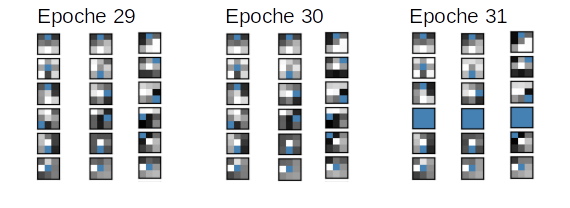
\includegraphics[width=0.9 \textwidth]{KapitelPartA/images/union.png}
 % union.png: 570x208 px, 96dpi, 15.08x5.50 cm, bb=0 0 427 156
 \caption{Beispielhafte Darstellung des Kanal-Union-Verfahrens}
 \label{abb:union}
\end{figure}



Zu diesem Zweck wird das Kanal-Union-Verfahren eingeführt. In Abbildung \ref{abb:channelUnion} wird beispielhaft ein Kanal-Union-Verfahren durchgeführt. Beim Kanal-Union-Verfahren wird eine Liste der Layer geführt, die aufeinander abgestimmt werden müssen. Im Falle eines residualen Netzes muss zusätzlich eine Liste der zusammengehörigen Layer der Kurzschlussverbindungen geführt werden. Im nächsten Schritt werden alle Eingangs- und Ausgangskanäle, die noch Gewichte größer Null haben in einer Liste gesammelt. Mit allen Elementen dieser Liste wird nun geprüft, ob mit Hilfe von Vereinigungen Kanäle gefunden werden können, die zwar keine von Null verschiedenen Gewichte mehr haben, wegen der Dimensionalität aber trotzdem beibehalten werden müssen. Alle Kanäle, die nicht unter diese Bedingung fallen, können mit Hilfe einer Rekonfiguration aus dem Netzwerk entfernt werden. In Abbildung \ref{abb:union} sind beispielhaft drei Eingangs- und sechs Ausgangskanäle dargestellt. In jedem Element des kartesischen Produkts der Menge der Eingangs- und Ausgangskanäle ist jeweils ein drei mal drei Felder großer Kernel dargestellt. Die Werte der Gewichte sind blau markiert, sobald sie absolut kleiner als der gewählte Grenzwert sind. Je dunkler die nicht-blauen Gewichte sind, desto kleiner sind sie. Da zwischen den jeweiligen Epochen für jede Batch eine Anpassung der Gewichte durchgeführt wird, entstehen teilweise große Veränderungen zwischen den Epochen. Dies ist zum Beispiel von Epoche 30 zu Epoche 31 im vierten Ausgangskanal sichtbar. Hier fällt innerhalb einer Epoche der Großteil des Ausgangskanal unter den Grenzwert.
\begin{figure}
\begin{minipage}[c]{1\linewidth}
\begin{tabularx}{1\textwidth}{m{0.2\textwidth}m{0.8\textwidth}} 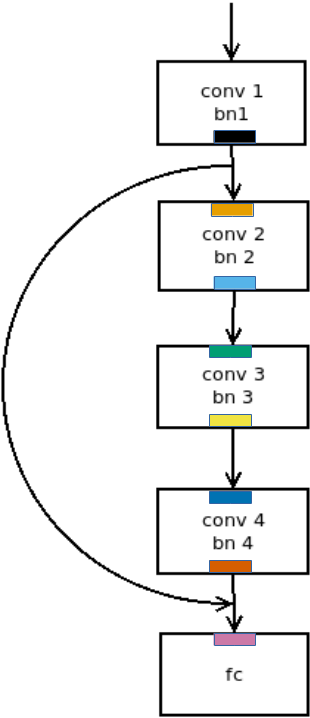
\includegraphics[width=0.21\textwidth]{KapitelPartA/images/net.png} &Liste der Layer, die direkt hintereinander sind und aufeinander abgestimmt werden müssen (ohne das zwischen den Layern eine Kurzschlussverbindung beginnt oder endet): $H=\left\{(\colorbox{sky}{2},\colorbox{bluegreen}{3}),(\colorbox{yellow}{3},\colorbox{blue2}{4}) \right\}$\newline
Liste der Layer, die im Zusammenhang mit den Kurzschlussverbindungen die gleiche Eingangskanaldimension haben müssen: \newline$E=\left\{(\colorbox{orange}{2},\colorbox{purple}{fc} \right\}$ \newline
Liste der Layer, die im Zusammenhang mit den Kurzschlussverbindungen die gleiche Ausgangskanaldimension haben müssen: $A=\left\{ ( \colorbox{black}{\textcolor{white}{1} },\colorbox{vermi}{4} ) \right\} $ \newline
Liste der dicht-besetzten Schichten vor dem ersten Beschneiden:\newline
$1:\left\{0,1,2\right\},\left\{\colorbox{black}{ \textcolor{white}{0,1,2,3,4,5,6,7}} \right\}$ \newline
$2:\left\{\colorbox{orange}{0,1,2,3,4,5,6,7}\right\},\left\{\colorbox{sky}{0,1,2,3,4,5,6,7}\right\}$\newline
$3:\left\{\colorbox{bluegreen}{0,1,2,3,4,5,6,7}\right\},\left\{\colorbox{yellow}{0,1,2,3,4,5,6,7}\right\}$\newline
$4:\left\{\colorbox{blue2}{0,1,2,3,4,5,6,7}\right\},\left\{\colorbox{vermi}{0,1,2,3,4,5,6,7}\right\}$\newline
$fc:\left\{\colorbox{purple}{0,1,2,3,4,5,6,7}\right\},\left\{0,1,2,3,4,5,6,7,8,9,10\right\}$ \newline

\\
\multicolumn{2}{m{1\linewidth}}{Liste der dicht-besetzten (db) Schichten nach dem 'auf-Null-setzen' der Parameter aber vor der Rekonfiguration:\newline
$1:\left\{0,1,2\right\},\left\{\colorbox{black}{\textcolor{white}{0,1,4,5,6,7}}\right\}$\newline
$2:\left\{\colorbox{orange}{0,1,3,5,6,7}\right\},\left\{\colorbox{sky}{0,1,2,4,5,6,7}\right\}$\newline
$3:\left\{\colorbox{bluegreen}{0,1,2,4,5,6,7}\right\},\left\{\colorbox{yellow}{0,1,2,3,5,6,7}\right\}$\newline
$4:\left\{\colorbox{blue2}{0,1,3,4,6,7}\right\},\left\{\colorbox{vermi}{0,1,3,4,5,6,7}\right\}$\newline
$fc:\left\{\colorbox{purple}{0,1,3,4,5,6}\right\},\left\{0,1,2,3,4,5,6,7,8,9,10\right\}$\newline
Vorgehen des Kanal-Union-Verfahrens:
Als erster Schritt wird für alle Elemente aus $H$ die Vereinigung von Ausgangs- und Eingangskanälen berechnet und diese dann zugewiesen:\newline
$\colorbox{sky}{2},\colorbox{bluegreen}{3}:A(\colorbox{sky}{2}) \cup E(\colorbox{bluegreen}{3})= \l\left\{\colorbox{sky}{0,1,2,4,5,6,7}\right\} \cup \left\{\colorbox{bluegreen}{0,1,2,4,5,6,7}\right\} =\left\{0,1,2,4,5,6,7\right\} $\newline
Hier wird der dünn-besetzte Kanal 3 entfernt \newline
$\colorbox{yellow}{3},\colorbox{blue2}{4}: A(\colorbox{yellow}{3}) \cup E(\colorbox{blue2}{4}) =
\left\{\colorbox{yellow}{0,1,2,3,5,6,7}\right\} \cup :\left\{\colorbox{blue2}{0,1,3,4,6,7}\right\} =\left\{0,1,2,3,4,5,6,7\right\}$\newline
Der nullwertige Eingangskanal 5 von Schicht 4 wird nicht entfernt, da der dazugehörige Ausgangskanal von Schicht 3 nicht nullwertig ist.
Im nächsten Schritt werden für die Elemente an jeweils gleicher Stelle aus den Mengen A und E Vereinigungen gebildet:
$A(\colorbox{black}{\textcolor{white}{1}})\cup A(\colorbox{vermi}{4}) \cup E(\colorbox{orange}{2}) \cup E(\colorbox{purple}{fc})=$\newline
$\left\{\colorbox{black}{\textcolor{white}{0,1,4,5,6,7}}\right\} \cup \left\{\colorbox{vermi}{0,1,3,4,5,6,7}\right\} \cup \left\{\colorbox{orange}{0,1,3,5,6,7}\right\} \cup \left\{\colorbox{purple}{0,1,3,4,5,6}\right\} = \left\{ 0,1,3,4,5,6,7\right\}$\newline
Hier wird in den Ausgangskanälen von Schicht 1 und 2 sowie in den Eingangskanälen von Schicht 2 und fc jeweils der 2. Kanal entfernt.}
\end{tabularx}
\end{minipage}
\caption{Beispielhafte Durchführung des Channel Union-Verfahrens}
\label{abb:channelUnion}
\end{figure}



Bei einem residualen Netzwerk kann weiterhin ein ganzer Block wegfallen. In diesem Fall müssen die Kanal-Union-Listen angepasst werden, die weitere Aktion wird ohne diesen Block im um mehrere Schichten verkürzten Netzwerk weiter geführt


Da mit dem Verkleinern des Netzes nicht nur potentiell Zeit sondern auch Speicherplatz gespart wird, kann bei gleicher Speicherauslastung die Batchgröße erhöht werden. Da die verwendete Technik für die Erhöhung der Batchgröße in der Quelle nicht angegeben ist und in der verwendeten Implementierung fehlt, wurde diese nachimplementiert. Dies wird in Kapitel \ref{sec:ptnew} erläutert \cite{ptImpl}. Hierbei wird die Lernrate an die erhöhte Batchgröße angepasst um negative Effekte für die Accuracy abzumildern oder auszuschließen. 

Damit lassen sich Netzverkleinerungsraten von etwa 50 \% erreichen bei weniger als 2 \% Accuracy-Verlust auf dem Datensatz Cifar10. Andere Techniken schaffen zwar zwischen 70 - 80 \% Netzverkleinerungsraten brauchen jedoch wesentlich mehr Trainingszeit \cite{lottery}. Diese großen Verkleinerungsraten sind dort sehr stark abhängig von der Initialisierung \cite{lottery}. Das heißt, nur einzelne Initialisierungen führen zu so starken Verkleinerungsraten, was insgesamt zu einer längeren Trainingszeit führt \cite{lottery}. 


Eine weitere Beschneidungstechnik arbeitet vor dem Training des Netzwerkes \cite{snyc}. Damit wird das Netz abhängig von der Initialbelegung beschnitten. Es lassen sich zwar sehr große Teile der Parameter auf Null setzen, hierbei wird im Vergleich zur Beschneidungsmethode während des Trainings allerdings weder für gemeinsames Beschneiden von Kanälen gesorgt, noch wird ein Rekonfigurationsverfahren vorgestellt. Somit hat das Netz am Ende des Verfahrens zwar relativ viele auf Null gesetzte Parameter ist aber weder schneller noch kleiner.


\section{Beschleunigung des Lernens durch Wissenstransfer}
\label{sec:net2net}
Beim Trainieren eines CNNs kommt es häufig vor, dass nach initialem Wählen der Tiefe beziehungsweise Breite des Netzes diese Parameter in einem weiteren Trainingslauf erhöht werden und in Folge dessen das Netzwerk komplett neu trainiert werden muss. Mit Hilfe der Quelle zu diesem Unterkapitel wurde ein Verfahren geschaffen, welches das Netz tiefer oder breiter machen kann und dabei die im ersten Trainingsdurchlauf trainierten Gewichte weiter verwendet \cite{net2net}. Durch diesen Wissenstransfer von einem Netz zu einem tieferen oder breiteren Netz wird eine schnellere Konvergenz des neuen Netzes erwartet. Durch die Initialisierung mit schon vorhandenen Parametern entsteht eine Transformation, die die erlernte Funktion erhält.

\begin{figure}[h]
 \centering
 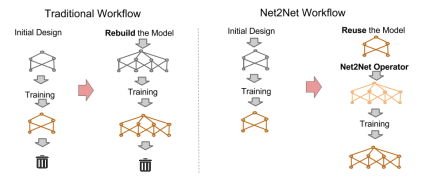
\includegraphics[width=0.7\textwidth]{KapitelPartA/images/net2net.png}
 % net2net.png: 433x179 px, 72dpi, 15.28x6.31 cm, bb=0 0 433 179
 \caption{Traditioneller Workflow vs. Net2Net Workflow}
 \label{abb:net2net}
\end{figure}


Wie in Abbildung \ref{abb:net2net} abgebildet ist, lässt sich so der Arbeitsablauf zum Finden der passenden Netzstruktur anders gestalten. Der Net2Net-Operator macht hier das Netz entweder breiter (mehr Kanäle in bestimmten Schichten) oder tiefer (zusätzliche Schichten). Diese beiden Operatoren werden nun vorgestellt.

\subsubsection{Operator für breiteres Netz}
Beim Operator für ein breiteres Netz werden für eine bestimmte Schicht Ausgangskanäle und für die nachfolgende Schicht Eingangskanäle hinzugefügt. Die Schicht, der die Ausgangskanäle hinzugefügt werden, wird mit $j$ bezeichnet und hat den Gewichtstensor $\mathbf{W}_j$ mit der Dimensionalität von $n \times l \times d(h_{l,1}) \times d(h_{l,2}$. Die Schicht, der die Eingangskanäle hinzugefügt werden wird mit $j+1$ bezeichnet und hat den Gewichtstensor $\mathbf{W}_{j+1}$ mit der Dimensionalität von $m \times n \times d(h_{j+1,1}) \times d(h_{j+1,2})$. Dem Layer $j$ werden $q$ Kanäle hinzugefügt. Dies entspricht wie in Abbildung \ref{abb:channels} abgebildet ist $q \cdot l $ zusätzlichen Kerneln. 
\begin{figure}[h]
 \centering
 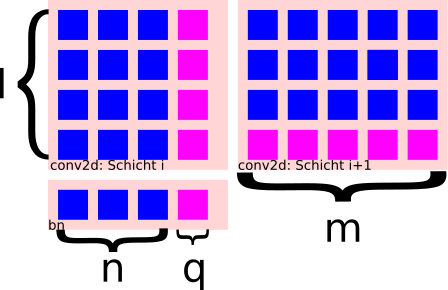
\includegraphics[width=0.6\textwidth]{KapitelPartA/images/channels.png}
 % channels.pdf: 0x0 px, 300dpi, 0.00x0.00 cm, bb=
 \caption{Übersicht über die zusätzlichen Kanäle}
\label{abb:channels}
 \end{figure}



Für den Layer $j+1$ sind es entsprechend $q \cdot m $ zusätzliche Kernel. Die Gewichtstensoren nach dem Anwenden des Net2Net-Operators werden mit $\mathbf{U}^j$ und $\mathbf{U}^{j+1}$ bezeichnet und sollen die Dimensionalität von $\mathbf{U}^j: (n+q) \times l \times d(h_{(j,1)}) \times d(h_{(j,2)})$ und $\mathbf{U}^{j+1}: m \times (n+q) \times d(h_{(j+1,1)}) \times d(h_{(j+1,2)})$ haben. Der Net2Net-Operator wird angewendet, indem zunächst eine Mapping-Funktion $g$ definiert wird, die für eine zufällige Belegung der zusätzlichen Kernels sorgt:

\begin{equation}
 g(j) =  
 \begin{cases}
 j & , \text{ falls} \, j \leq n \\
 k & , \text{ falls} \, j>n : \;  k \text{ zufälliges Sample von} \left\{ 1,2,\ldots, n \right\} \\ 
 \end{cases} 
 \end{equation}
 Mit Hilfe dieser Mapping-Funktion werden nun die neuen Gewichtstensoren initialisiert:
 \begin{align*}
 \mathbf{U}_j(e,f,h_{j,1},h_{j,2}) &= \mathbf{W}_j(g(e),f,h_{j,1},h_{j,2}) \\
 \mathbf{U}_{j+1}(e,f,h_{j+1,1},h_{j+1,2})&= \frac{1}{|\left\{ x | g(x)=g(a)\right\}|}\mathbf{W}_{j+1}(e,g(f),h_{j+1,1},h_{j+1,2})
 \end{align*}
Die Funktion $g(j)$ wird dabei für jede neu hinzugekommene Schicht nur einmal ausgewertet, sodass gesamte Reihen statt einzelner Kernel kopiert werden. Sollte sich zwischen dem $j$-ten und $(j+1)$-Layer eine Batchnormalisierungsschicht befinden, so werden die Parameter dieser Schicht ebenfalls kopiert.

Um nicht mehrere exakt gleiche Kernelreihen zu haben kann außerdem noch ein Noiseanteil auf alle Gewichte addiert werden. Dies ist vor allem für den Fall wichtig, wenn der Trainingsalgorithmus keine Form der Randomisierung hat, das heißt die gleichen Gewichtstensoren werden ermutigt, unterschiedliche Funktionen zu erlernen. Somit sind die vom ursprünglichen und neuen Netz gelernten Funktionen ähnlich aber nicht gleich.

\subsubsection{Tieferes Netz}

Der Operator für ein tieferes Netz ersetzt die Operation der $j$-ten Schicht $\mathbf{v}_{i,j} = \text{BN}_{\gamma,\beta}( \mathbf{v}_{i,j}* \mathbf{W}_{j})$ durch die Operation von zwei Layern  
\begin{equation}
\mathbf{v}_{i,j} =\text{BN}_{\gamma',\beta'}( \text{BN}_{\gamma,\beta}( \mathbf{v}_{i,j} * t(W_{j})) * t(U_{j})    )
\end{equation}
$\mathbf{U}$ wird als Identitätsmatrix initialisiert.
Da zwischen den beiden Layern eine Batchnormalisierung genutzt wird, müssen die Parameter der Batchnormalisierung $\gamma'$ und $\beta'$ so gewählt werden, dass sie die gelernte Funktion des Netzes nicht verändern.


\subsubsection{Diskussion der Methode}

Die beiden Net2Net-Operatoren schaffen die Möglichkeit, Familien von Netzarchitekturen zu erforschen ohne jedes Mal von neuem zu lernen. Mit Hilfe der beiden Operatoren lässt sich die Komplexität des Netzes erhöhen ohne die gelernte bisherige Funktion zu vernachlässigen.




\section{Automatische Architektursuche}\label{sec:auto}
Neben dem im letzten Kapitel ausführlich erläuterten Ansatz des Strukturlernens gibt es noch einige andere aktuelle Ansätze, die automatisch nach einer besseren Architektur für einen Datensatz suchen. Einige dieser Ansätze werden hier beleuchtet und es wird gezeigt, wieso das im letzten Kapitel erläuterte Verfahren im praktischen Teil weiter verwendet wird.

Beim Versuch die Hyperparameter eines Netzes sinnvoll automatisch zu wählen, entsteht ein sehr großer Suchraum. Dieser Suchraum lässt sich mit viel Aufwand absuchen \cite{dvolver}. Es entsteht ein Optimierungsproblem mit mehreren zu optimierenden Variablen bei welchem eine Pareto-Front gesucht wird \cite{dvolver}. Das Ergebnis schafft eine Verbesserung der Accuracy gegenüber bekannten Architekturen, dabei summiert sich allerdings die Trainingszeit mit 20 NVIDIA V100 Grafikkarten für Imagenet auf 2,5 Tage\cite{dvolver}.
Eine weitere Methode den Suchraum zu durchsuchen sind genetisch inspirierte Suchalgorithmen \cite{gen}. Dabei wird initial eine Population von Netzen gebildet \cite{gen}. Nach einem Trainingsdurchgang werden diese nach ihrer Fitness (Klassifikationsleistung) selektiert \cite{gen}. Im weiteren Verlauf werden jeweils zwei dieser Netze gepaart und es entsteht eine neue Generation an Netzen \cite{gen}. Allerdings ist hier die Trainingszeit in einem Rahmen von 35 GPUs für einen Tag \cite{gen}. Dann ist die Architektursuche allerdings komplett automatisiert und erreicht eine Accuracy von 96.78 \% für Cifar 10 und 79.77 \% für Cifar 100 \cite{gen}. \footnote{Um diese Zahl einordnen zu können: die besten zehn Accuracy-Werte liegen für Cifar 10 bei 96.62 \% bis 99.37 \% und für Cifar 100 bei 82,35 \% bis 93,51 \%. Entsprechende Veröffentlichungen sind unter \url{https://benchmarks.ai/} zu finden}  

Das Ziel von einigen Veröffentlichungen im Themenbereich der automatischen Architektursuche ist es, diese lange Trainingszeit zu reduzieren.

Eine Möglichkeit der Reduzierung bietet sich durch Ausnutzung von domainspezifischen Eigenschaften der zu klassifizierenden Bilder. Eine Möglichkeit einer domainspezifischen Eigenschaft, die genutzt werden kann, ist, wenn die Bilder nicht klassisch mit einer Kamera, sondern mit anderen Geräten aufgenommen wurden. Diese veränderte Aufnahmeart kann dafür sorgen, dass sich der Suchraum massiv einschränken lässt und sich damit die Architektursuche beschleunigt.
Als Beispiel kann hier eine Radaranlage zur Aufnahme von Bilder dienen \cite{polsar}.


Eine weitere Möglichkeit die Trainingszeit zu minimieren ist es, den Suchraum deutlich zu verkleinern und die Anzahl an Durchläufen zu minimieren. Der Nachteil ist dann allerdings, dass die Wahrscheinlichkeit, ein Netz in einem globalen Optimum zu finden bezüglich des Suchraumes klein ist. Eine Methode die dies nutzt, wird im nächsten Unterkapitel vorgestellt.

\section{Schnelles Ressourcen-beschränktes Strukturlernen tiefer Netzwerke}\label{sec:morphnet}
Im Gegensatz zu den Kapiteln \ref{sec:prunetrain} und \ref{sec:net2net}, in denen jeweils eine Möglichkeit, ein CNN kleiner sowie größer zu machen vorgestellt wurden, geht es jetzt darum, dies zu kombinieren. Die Quelle für diese Kapitel ist, soweit nicht anders gekennzeichnet, das Paper, welches die Methode vorgestellt hat.

Die manuelle Wahl von Hyperparametern, die bestimmen wie groß und komplex ein neuronales Netz ist, 
braucht Erfahrung und Kunstfertigkeit. Sind die Hyperparameter falsch gewählt, so müssen diese angepasst und das Netz erneut trainiert werden. Mit Hilfe der hier vorgestellten Methode wird die Suche nach der besten Architektur automatisiert. Dies geschieht mit Hilfe von iterativen Verkleinern und Vergrößern des Netzes. Diese Methode hat drei Vorteile:
\begin{enumerate}
 \item Es ist auf große Netze und große Datensätze skalierbar
 \item Es kann die Struktur in Bezug auf eine bestimmte Nebenbedingung (zum Beispiel Modellgröße, Anzahl an Parametern) optimieren
 \item Es kann eine Struktur lernen, die die Performance erhöht
\end{enumerate}

Das Ziel der Methode ist es, automatisch die beste Architektur für ein Netz zu finden. Dies umfasst die Breiten der Eingangs- und Ausgangskanäle, Größe der Kernel, die Anzahl der Schichten und die Konnektivität dieser Schichten. Im Rahmen dieser Methode wird dies auf die Breite der Ausgangskanäle eingeschränkt. Die Methode kann auf die anderen Größen erweitert werden. Allerdings ist die Einschränkung auf die Breite der Ausgangskanäle sowohl effektiv als auch simpel.
Die Breite der Ausgangskanäle für alle $J$ Schichten wird mit $\mathcal{C}_{1:J}$ bezeichnet. 

Der Anfangspunkt dieser Methode ist ein Netz $\mathcal{W}^1$ mit einer initialen Breite der Ausgangskanäle sowie fixen Filtergrößen. Die Nebenbedingung wird mit der Funktion $\mathcal{F}$ bezeichnet. Sie optimiert entweder die Modellgröße oder die Anzahl an Flops per Inferenz. Die Methode optimiert formal gesehen also folgendes:
\begin{equation}
 \mathcal{W}^{\ast}= \underset{\mathcal{F}(\mathcal{C}_{1:J})\leq \zeta}{\text{arg min}} \underset{\mathcal{W},\mathbf{x}_i \in \mathcal{B}}{\text{ min}}\; l(f(\mathbf{x_i}, \mathcal{W}),y_i)\label{equ:morph1}
\end{equation}

Das Vergrößern des Netzes basiert auf einer Lösung für die Gleichung \ref{equ:morph1}: dem Breitenmultiplikator $\omega$. 
Sei $\omega \cdot O_{1:M} = \left\{ \lfloor \omega O_1 \rfloor, \lfloor \omega O_2 \rfloor, \ldots , \lfloor \omega O_M \rfloor \right\}, \omega>0$. Gilt $\omega>1$, so wird das Netz vergrößert. Bei $\omega <1$ wird das Netz verkleinert. Um die Gleichung \ref{equ:morph1} zu lösen, finde nun das größte $\omega$, so dass $\mathcal{F}(\omega \cdot O_{1:M})\leq \zeta$ gilt.


Dieser Ansatz sorgt für eine mögliche Verkleinerung und Vergrößerung des Netzes und er funktioniert gut bei einem guten initialen Netz. Ist das initialen Netz aber nicht von so guter Qualität, so hat dieser Ansatz Probleme. Grund hierfür ist wahrscheinlich ein lokales Minimum, aus welchem die Optimierungsfunktion nicht mehr herausfindet, um ein besseres lokales oder globales Minimum zu finden.

Dieser Nachteil wird durch eine Veränderung der Verlust-Funktion aufgehoben. Es wird ein Regularisierer $\mathcal{G}$ dazu addiert, welcher misst, wie groß der Anteil eines Netzbestandteiles an $\mathcal{F}( \mathcal{C}_{1:J})$ ist, und der es damit direkt optimieren kann. Dann ist
\begin{equation}
 W^{\ast}= \underset{\mathcal{F}(\mathcal{C}_{1:J})\leq \zeta}{\text{arg min}} \underset{\mathcal{W}}{\text{min}}\; l(f(\mathbf{x_i}, \mathcal{W}),y_i) + \lambda \mathcal{G}( \mathcal{W})  
 \label{equ:morph2}
\end{equation}
Dieser Ansatz kann die relative Größe einer Schicht ändern, hat aber den Nachteil das häufiger die zu optimierende Nebenbedingung nicht optimal maximiert wird.


Die beiden Ansätze lassen sich kombinieren. Algorithmus \ref{alg:morphnet} beschreibt den Algorithmus der bei der Kombination entsteht mit Pseudocode.
\begin{algorithm}[H]
\caption{MorphNet Algorithmus}
\begin{algorithmic}[1]
\STATE Trainiere das Netz um $\mathcal{W}^{\ast}=\underset{\mathcal{W}}{arg min}\; l(f(\mathbf{x_i}, \mathcal{W},y_i) + \lambda \mathcal{G}(\mathcal{W}))$ zu finden
\STATE Finde die neue Breite $\mathcal{C}_{1:J}^{\prime}$, die durch 1. errechnet wurde
\STATE Finde das größte $\omega$, so dass $\mathcal{F}(\omega \cdot \mathcal{C}_{1:J})\leq \zeta$ gilt
\STATE Wiederhole ab 1. so häufig wie gewünscht mit $\mathcal{C}_{1:J} = \mathcal{C}_{1:J}^{\prime}$
\ENSURE $\omega \cdot \mathcal{C}_{1:J}$
\end{algorithmic}
\label{alg:morphnet}
\end{algorithm}
Dieser Algorithmus kann so oft durchlaufen werden bis entweder die Performance des Netzes gut genug ist, oder bis die letzten Durchläufe keine Veränderungen mehr hervorgebracht haben.


\subsection{Definition der Nebenbedingung}
Die Nebenbedingung $\mathcal{F}$ lässt sich für verschiedene zu optimierende Zielgrößen definieren. Eine einfache Nebenbedingungen, die Modellgröße wird hier beispielhaft erläutert. Die Größe dieser Nebenbedingung wird vor allem durch Schichten mit Matrixmultiplikation dominiert. Die Modellgröße ergibt sich durch die Größe der Tensoren der einzelnen Schichten. Da die Größe der Tensoren der einzelnen Schichten abhängig von der Anzahl der Eingangs- und Ausgangskanäle sowie der Filtergröße und nicht von der Position im Netzwerk ist, lässt sich $\mathcal{F}(\mathcal{C}_{1:J})$ auf die einzelnen Schichten zurückführen. Es gilt:
\begin{equation}
 \mathcal{F}(\mathcal{C}_{1:J})=\sum_{j=1}^{J} \mathcal{F}(j)
\end{equation}
Für den Breitenmultiplikator $\omega$ gilt: $\mathcal{F}(\omega \cdot \mathcal{C}_{1:J}=\sum_{j=1}^{J} \omega \cdot \mathcal{F}(j)$

Die Abhängigkeit von der Größe des jeweiligen Tensors ergibt für 
\begin{equation}\label{equ:F}
\mathcal{F}(j)=c_j \cdot k_j \cdot d(h_{j,1}) \cdot d(h_{j,2})  
\end{equation}
Da durch die Anwendung des Regularisierers einzelne Kanäle auf Null gesetzt werden und ein Netz ohne diesen Kanal möglich wäre, sollen diese Kanäle in dieser Berechnung ausgelassen werden. Daher wird die Formel um Aktivierungsfunktionen $A_{k_l,j}$ und $B_{c_l,j}$ ergänzt die mit einer Eins angeben, dass der zugehörige Kanal nicht null ist. Eine Null als Ergebnis der Aktivierungsfunktion ergibt sich, wenn der entsprechende Kanal komplett auf Null gesetzt wurde. Dadurch lassen sich $c_j$ und $k_j $ aus Formel \ref{equ:F} ersetzen:
\begin{equation}
\mathcal{F}(j)=\left(\sum_{k=1}^{k_l} A_{k,j} \right) \cdot \left(\sum_{c=1}^{c_l} B_{c,j}\right) \cdot d(h_{j,1}) \cdot d(h_{j,2})  
\end{equation}


\subsection{Regularisierer}
Beim Verkleinern des Netzes soll die Verlustfunktion $l$ des CNN mit der Nebenbedingung $\mathcal{F}(\mathcal{C}_{1:J})\leq \zeta$ minimiert werden. Bei der Wahl des Regularisierers muss bedacht werden, dass der Regularisierer und seine Ableitung kontinuierlich definiert sein müssen, da die Parameter im Netz durch ein Gradientenabstiegsverfahren gelernt werden. Zusätzlich kann eine Nebenbedingung nicht direkt durch ein Gradientenabstiegsverfahren gelernt werden. Daher wird $\mathcal{F}$ in veränderter Form als Regulariser gewählt. Die Veränderung umfasst das Hinzufügen von $\gamma$, die ähnlich einer Batchnormalisierung genutzt werden:
\begin{equation}
\mathcal{G}(j)=\left(\sum_{k=1}^{k_l-1} A_{k_l,j} \sum_{c=1}^{c_l-1} |\gamma_{c, j} | \right) \cdot \left(\sum_{k=1}^{k_l-1} |\gamma_{k,j} |   \sum_{c=1}^{c_l-1} B_{c,j}\right) \cdot d(h_{j,1}) \cdot d(h_{j,2})  
\end{equation}

Mit dieser Funktion lässt sich mittels Gradientenabstieg lernen, obwohl Teile des Regularisieres nicht komplett kontinuierlich sind. $\gamma$ muss dabei kontinuierlich sein. Werden die $\gamma$ für einen Kanal auf Null gesetzt durch das Lernen, so ist der dazugehörige Kanal aus der Berechnung wie gewünscht ausgeschlossen. Für jeden Ein- und Ausgangskanal einer Schicht wird ein $\gamma$ in den Vorwärts-Durchgang eingebaut. Diese Parameter funktionieren dann analog zu den $\gamma$ aus der Batchnormalisierung, da sie kontrollieren, welcher Prozentsatz eines Kanals weitergeleitet wird.


Aus dem Regularisierer einer Schicht lässt sich mittels Addition die Regularisierung des kompletten Netzes berechnen.
\begin{equation}
 \mathcal{G}(\mathcal{W})=\sum_{j=1}^{J} \mathcal{G}(j)
\end{equation}


Um die Wichtigkeit vom besseren Training des Netzes und der Regularisierung von Parametern treffen zu können wird ein Parameter $\lambda$ eingeführt. So entsteht die Verlust-Funktion
\begin{equation}
 \mathcal{W}^{\ast}=\underset{\mathcal{W}}{arg min}\; \; l(f(\mathbf{x}_i, \mathcal{W}),y_i) + \lambda \mathcal{G}(\mathcal{W})
\end{equation}



Dieser Regularisierer funktioniert nicht für Netze, die Kurzschlussverbindungen besitzen. Hier wird, wie beim Beschneiden des Netzes während des Trainings, ein Gruppen-Lasso verwendet. Dies stellt sicher, dass an Kurzschlussverbindungen nur so beschnitten werden kann, wie es für die Dimensionalität des Netzes zuträglich ist.







\section{Verringerung der für Berechnungen nötige Zeit}

Die Zeit, die ein Convolutional Layer braucht um berechnet zu werden hängt ab von:
\todo{Fehlt hier noch etwas?}
\begin{itemize}
 \item der Filtergr\"osse
 \item der Bildgr\"osse
 \item dem verwendeten Zahlenformat
\end{itemize}
Beim Verändern der Filter- oder der Bildgr\"osse, um Trainingszeit zu sparen, ver\"andert sich auch die Erkennungsleistung \todo{cite}. Dies ist beim Verändern des verwendeten Zahlenformats nicht umbedingt gegeben. Standardformat ist eine 32 Bit Gleitkommazahl. Die einfachste Methode hier Trainingszeit zu sparen ist das Halbieren der Bitanzahl auf 16 Bit. Eine weitere Methode ist das Benutzen von 16 Bit Dynamischen Festkommazahlen.
Die beiden alternativen Methoden haben unterschiedliche Anforderungen an die Ausführungsplattform. Diese Anforderungen und die Besonderheiten der beiden Verfahren werden in den folgenden zwei Unterkapiteln näher beleuchtet.


\subsection{Berechnung mit 16 Bit Gleitkomma}

Die 16 Bit Gleitkommazahl unterscheidet sich nicht nur in der Länge von der 32 Bit Zahl sondern aus der unterschiedlichen Länge erwachsen Unterschiede in den darstellbaren Zahlen. In Tabelle \todo{ref} sind diese Unterschiede dargestellt.





Diese Nachteile von 16 Bit Gleitkommazahlen können durch drei Techniken abgemeildert oder sogar komplett aufgehoben werden:
\begin{itemize}
 \item 32 Bit Mastergewichte und Updates
 \item Sklaierung der Loss-Funktion
 \item Arithmetische Präzision 
\end{itemize}

Diese drei Techniken werden in den drei folgenden Unterkpaiteln behandelt.

\subsubsection{32 Bit Mastergewichte und Updates}

Beim Trainieren von neuronalen Netzwerken mit 16 Bit Gleitkommazahlen werden die Gewichte, Aktivierungen und Gradienten im 16 Bit Format gespeichert. Die Speicherung der Gewichte als 32 Bit Mastergewichte hat zwei mögliche Erklärungen, die aber nicht immer zutreffen müssen. 

Um nach einem Forward Druchlauf des Netzes die Gewichte abzudaten wird ein Gradientenabstiegsverfahren benutzt. Hierbei werden die Gradienten der Gewichte berechnet. Um für die Funktion, die das CNN approximiert einen besseren Approximationserfolg zu erlangen wird dann dieser Gradient mit der Lernrate multipliziert. Wird dieses Produkt in 16 Bit abgespeichert, so ist in viele Fällen das Produkt der beiden Zahlen gleich Null. Dies liegt an der Taqtsache, dass wie in Tabelle \todo{ref} zu sehen ist die kleinste darstellbare Zahl in 16 Bit wesentlich grösser ist als in 32 Bit.


Der zweite Grund wieso man Mastergewichte brauchen könnte ist die Tatsache, dass bei grossen Gewichten die Länge der Mantisse nicht ausreicht, um sowohl das Gewicht als auch das zu  addierende Update zu speichern.

Aus den beiden Gründen wird das in Abbildung \todo{ref} gezeigte Schema zum Trainieren einer Schicht mit gemischt präzisen Gleitkommazahlen benutzt.

\missingfigure{Schema}

\subsubsection{Sklaierung der Loss-Funktion}

\subsubsection{Arithmetische Präzision}


\subsection{Berechnung mit 16 Bit Dynamischen Festkommazahlen}


Quelle: \cite{FPGpu}


\subsection{Beschleunigung der Berechnung des Gradientenabstiegsverfahren}
\todo[inline]{Überblick schreiben; 4 Stunden}
Bei der Beschleunigung der Berechnung des Gradientenabstiegsverfahren gibt es vier verschiedene publizierte Herangehensweisen:
\begin{itemize}
 \item Accelerating CNN Training by Sparsifying Activation Gradients
 \item Weight Normalization: A Simple Reparameterization
to Accelerate Training of Deep Neural Networks
 \item Accelerating Deep Neural Network Training with Inconsistent Stochastic Gradient Descent
 \item Accelerated CNN Training Through Gradient Approximation 
\end{itemize}


\subsubsection{Accelerating CNN Training by Sparsifying Activation Gradients}

\subsubsection{Weight Normalization: A Simple Reparameterization
to Accelerate Training of Deep Neural Networks}




\subsubsection{Accelerating Deep Neural Network Training with Inconsistent Stochastic Gradient Descent}



\subsubsection{Accelerated CNN Training Through Gradient Approximation }




\section{Additive Methoden}
Die Methoden in diesem Kapitel beeinflussen die Trainingszeit nicht direkt, sondern helfen die Folgen anderer Verfahren abzumildern.

\subsection{Ghost Batch Normalization}





\cleardoublepage
\chapter{Einleitung}
\label{sec:EinleitungGesamt}

\section{Motivation und Hintergrund dieser Arbeit}


MorphNet ist eine Möglichkeit mittels Verkleinern und Vergrössern des Netzwerkes effizient die Struktur eines Netzwerks zu lernen. Ist dieses Konzept auch auf PruneTrain zu übertragen und so zu erweitern, dass nicht das komplette Netz erweitert wird, sondern eben nur sinnvolle Bereiche?
Ist dieser Prozess mit Hilfe weiterer Methoden beschleunigbar?

\todo[inline]{Einleitung fertigschreiben -- zum Schluss}

\section{Aufbau der Arbeit}
\todo[inline]{Aufbau der Arbeit -- erst bei fortgeschrittener Arbeit schreiben}


\section{Suchbegriffe}
\todo[inline]{verwendete Suchbegriffe}


\chapter{Untersuchung von MorphNet}\label{sec:morphexperimente}

Die in Kapitel \ref{sec:morphnet} erläuterte Methode zum ``schnellen Ressourcen beschränkten Strukturlernen'' (MorphNet) wird in diesem Kapitel evaluiert. In Algorithmus \ref{alg:morphnet} wurde das Vorgehen von MorphNet mittels Pseudocode dargestellt. Im ersten Schritt zur Evaluierung werden die einzelnen Schritte in diesem Algorithmus evaluiert. Im zweiten Schritt wird überprüft, wie gut der Algorithmus auf dem Datensatz Cifar10 trainiert auf einem ResNet abschneidet.
Da als Framework Pytorch verwendet wird kann die ursprüngliche Implementation hier nicht verwendet werden. Es ist nicht sehr sinnvoll zwei Verfahren zu vergleichen, die auf unterschiedlichen Frameworks aufbauen. Stattdessen wird die im Rahmen einer anderen Veröffentlichung erstellte Implementierung vom MorphNet benutzt\footnote{Die benutzte Implementierung ist auf Github zu finden: \url{https://github.com/cmu-enyac/LeGR/} } \cite{morphImple}. Unterschiede in der Implementierung sollten hier theoretisch nicht vorliegen, da der originale Programmcode von MorphNet verfügbar ist\footnote{Der original Programmcode ist ebenfalls auf Github zu finden: \url{https://github.com/google-research/morph-net}}.

\section{Evaluierung der einzelnen Schritte von MorphNet}
Im ersten Schritt von MorphNet wird das Netz trainiert, so dass
\begin{equation}
\mathcal{W}^{\ast}=\underset{\mathcal{W},\mathbf{x}_i \in \mathcal{B}}{arg min}\; l(f(\mathbf{x_i}, \mathcal{W},y_i) + \lambda \mathcal{G}(\mathcal{W}))
\end{equation}
minimiert wird. Der Regularisierer $\mathcal{G}$ ist in dieser Formel dafür zuständig, dass die gewählte Zielgröße minimiert wird. Die zwei möglichen Zielgrößen sind die Modellgröße und Anzahl an FLOPs. Für beide Zielgrößen gilt, dass die im Regularisierer verwendete Formel nur eine vereinfachte Form der Zielgröße berechnet. 
Deshalb wird zunächst evaluiert, welchen Effekt der Regularisierer auf die Zielgröße hat. Dabei werden nur die ersten beiden Schritte des MorphNet-Algorithmus durchgeführt.


In Abbildung \ref{abb:morphFLOPs} ist in Grün abgebildet, wie sich der Wert des Regularisieres für die Zielgröße FLOPs während dem Training verändert. Die blaue Kurve in Abbildung \ref{abb:morphFLOPs} ist der tatsächliche Verlauf der Flops über die Trainingszeit. Die blaue Kurve wird in Schritten weniger, da das Netz nur alle fünf Epochen mittels der zweiten MorphNet-Schrittes beschnitten wird. Die verzögerte Reduzierung der Zielgröße liegt daran, dass erst mit einer gewissen Anzahl entfernbarer Gewichte tatsächlich eine Änderung an den FLOPs passiert. Für die Zielgröße Modellgröße ist der Verlauf der beiden Kurven in Abbildung \ref{abb:morphSize} abgebildet. Für die Zielgröße Modellgröße muss $\lambda$ größer sein um einen Effekt auf die Zielgröße zu haben. Es zeigt sich, dass $\mathcal{G}$ tatsächlich für eine minimierte Zielgröße sorgt.

\begin{figure}
     \centering
     \subfloat[][]{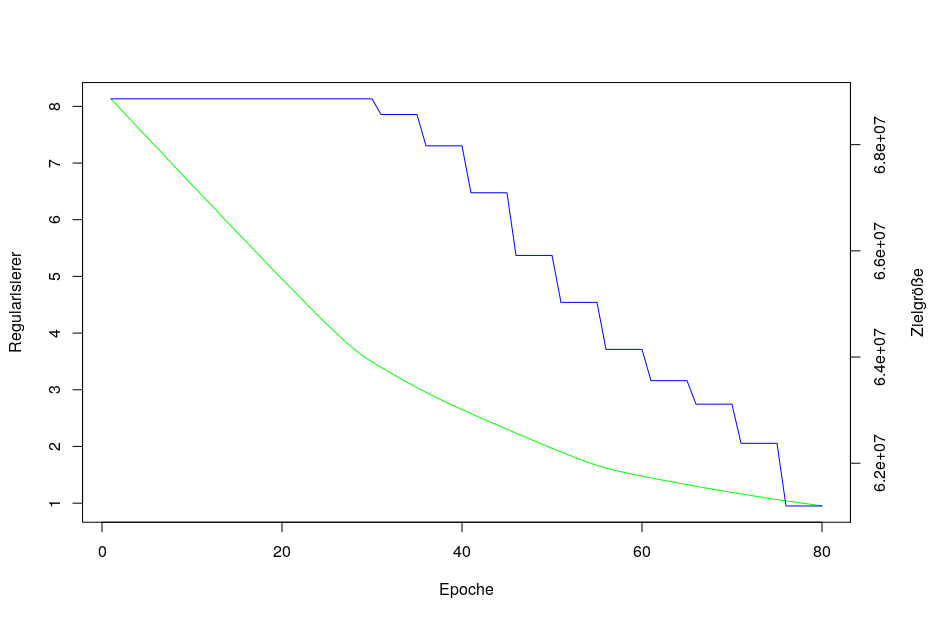
\includegraphics[width=0.47\textwidth]{KapitelPartB/Images/morph1.png}\label{abb:morphFLOPs}}
     \hfill
     \subfloat[][]{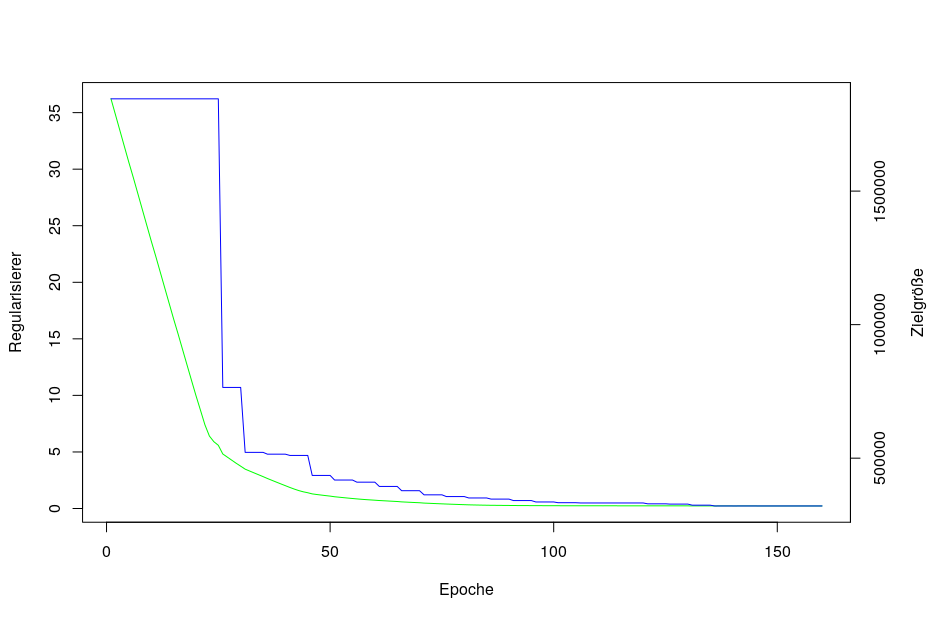
\includegraphics[width=.47\linewidth]{KapitelPartB/Images/morph2.png}\label{abb:morphSize}}
     \caption{Vergleich Zielgröße mit Wert des Regularisierers für (a) FLOPs (b) Modellgröße }
     \label{abb:morph1}
\end{figure}


Der Effekt von verschieden großen $\lambda$ wird im nächsten Schritt untersucht. Zu diesen Zweck wird ein Netzwerk mit verschiedenen Werten für $\lambda$ trainiert. Dabei wird das Netz jeweils für 180 Epochen trainiert und anschließend wird das Netz beschnitten. Abhängig von der Größe von $\lambda$ wird dem Regularisierer mehr oder weniger Gewicht gegeben. In Abbildung \ref{abb:morph3} ist zu sehen, wie sich der MorphNet Algorithmus bei verschiedenen $\lambda$ für die Zielgröße FLOPs verhält. In Abbildung \ref{abb:morph4} ist abgebildet wie sich die Netzverkleinerungsraten verändern, bei der Zielgröße Modellgröße. In der Originalveröffentlichung wurde der Effekt von verschiedenen $\lambda$ untersucht und für die Zielgröße FLOPs auch dargestellt. Dabei zeigte sich, dass mit verschiedenen Werten von $\lambda$ eine Kurve gebildet werden konnte, die für das Verhältnis zwischen Flops per Inferenz und der Accuracy einen Zusammenhang findet: Je kleiner die Flops Anzahl ist, so geringer ist auch die Accuracy \cite{morphnet}. Wie in Abbildung \ref{abb:morph3} für die Zielgröße Flops zu sehen ist, ist dieser Zusammenhang für ein ResNet nicht zu finden. Die Accuracy der hier angegebenen Netze ist im so gering, da viel vom Netz weggeschnitten wird, beziehungweise durch den Regularisierer minimiert wurden. Durch die große Verkleinerungsrate sind auch größere Veränderungen an der Struktur möglich.


In Abbildung \ref{abb:morph5} ist abgebildet, wie sich die Zielgröße Flops im Zusammenhang mit der Accuracy verändert, bei einem festen $\lambda = 3 \cdot 10^{-8}$. Im Vergleich zeigt sich jetzt das in Abbildung \ref{abb:morph4} für mehrere verschiedene $\lambda$ eine Accuracy Spanne von 6.43 \% ergibt. Bei $\lambda = 3 \cdot 10^{-8}$ ergibt sich eine Spanne von 5,72 \%. Damit zeigt sich, dass das Ergebnis nach einem Beschneidungsvorgang nicht stabil ist. Dies könnte an der generellen Instabilität des Trainings liegen (stark sich verändernde Accuracy- Werte) oder an strukturellen Unterschieden zum Inception Netz. Wie in Kapitel \ref{sec:inception} geschrieben unterscheidet sich das ResNet vom Inception Netz durch das Fehlen von Kurzschlussverbindungen, das Anwenden mehrere Filter im Inception Netz und der Tiefe vom Inception Netz. Ein weiterer Unterschied, der für das unterschiedliche Abschneiden verantwortlich sein. könnte ist die Verwendung von Cifar 10 statt Imagenet.


In Tabelle \ref{tab:time} sind die durchschnittlichen Trainingszeiten für die Zielgröße FLOPs im Vergleich mit dem Baseline-Netz zu sehen. Der Unterschied zwischen den verschiedenen Werten von $\lambda$ zeigt und dem breiten Baseline-Netz zeigt, dass etwa 3,5 Sekunden zwischen der durchschnittlichen Trainingszeit des Baseline-Netzes und den durchschnittlichen Trainingszeiten von MorphNet mit den vier verschiedenen $\lambda$. Da hier nur einmal beschnitten wird hauptsächlich gemessen, wie viel Overhead durch das Berechnen des Regularisierers entsteht.
\begin{table}[]
\begin{tabular}{c|c|c|c|c|c|}
\cline{2-6}
                                                      & Baseline & $1\cdot 10^{-8}$   & $2\cdot 10^{-8}$   & $3\cdot 10^{-8}$   & $4\cdot 10^{-8}$   \\ \hline
\multicolumn{1}{|l|}{durchschnittliche Trainingszeit} & 19,57    & 23,13 & 23,03 & 23,07 & 23,10 \\ \hline
\end{tabular}
\caption{Durchschnittliche Trainingszeiten verschiedener $\lambda$ und dem Baseline-Netz}
\label{tab:time}
\end{table}

\begin{figure}
     \centering
     \subfloat[][]{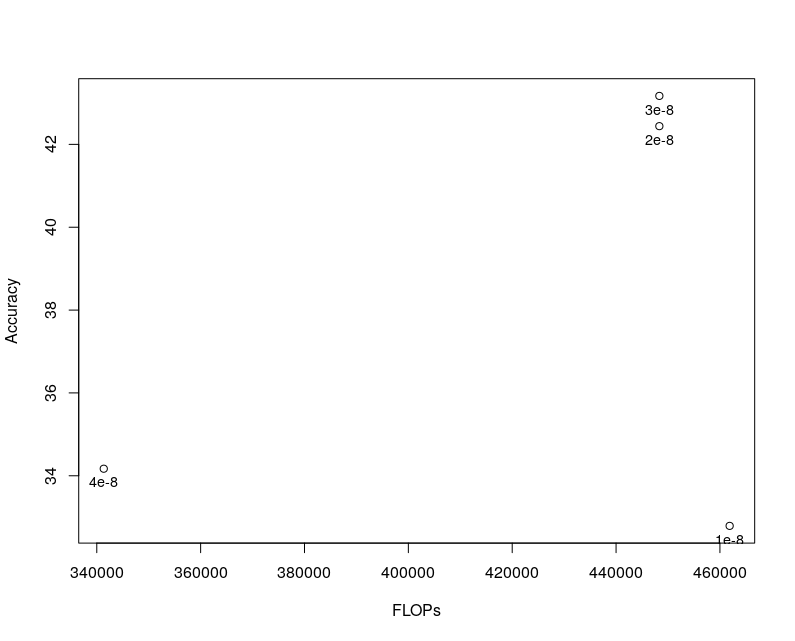
\includegraphics[width=0.47\textwidth]{KapitelPartB/Images/morph3.png}\label{abb:morph3}}
     \hfill
     \subfloat[][]{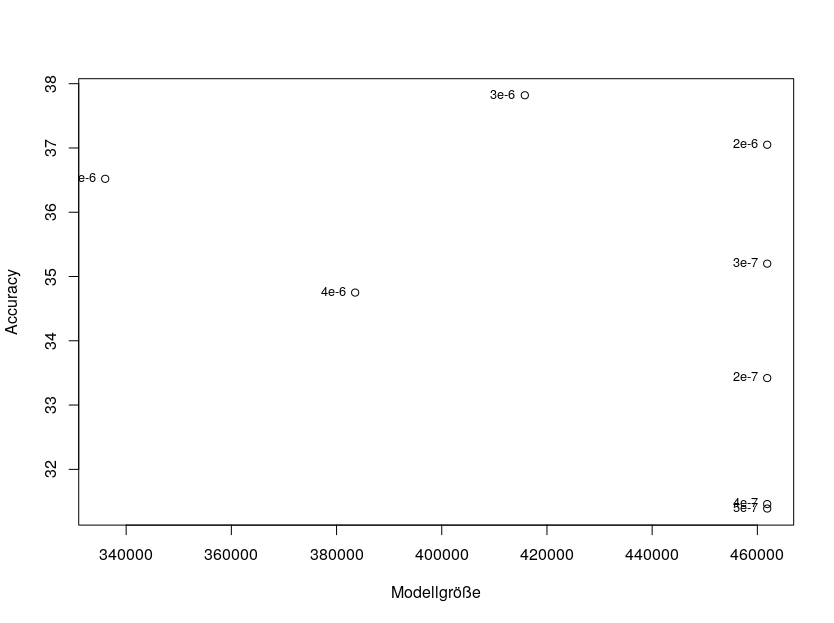
\includegraphics[width=.47\linewidth]{KapitelPartB/Images/morph4.png}\label{abb:morph4}}
     \subfloat[][]{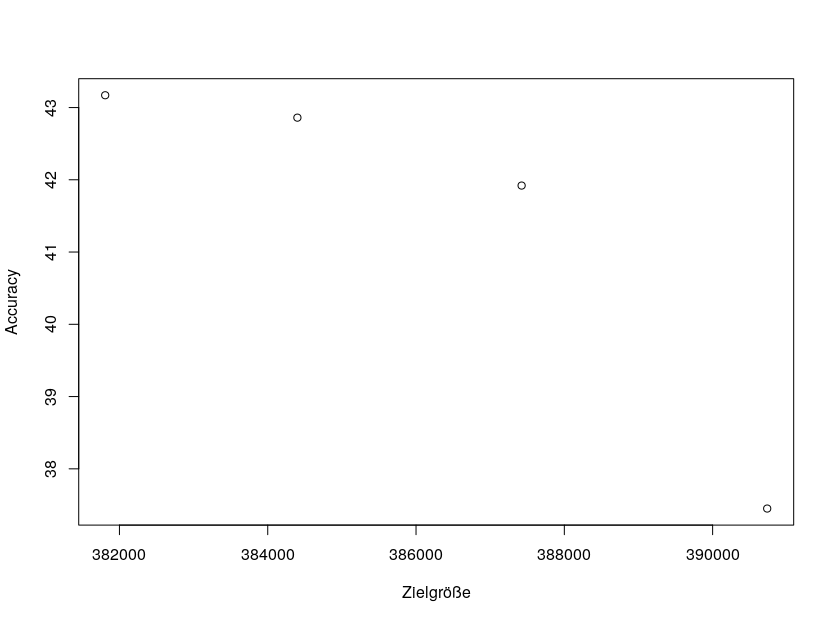
\includegraphics[width=.47\linewidth]{KapitelPartB/Images/morph5.png}\label{abb:morph5}}
     \caption{Effekt verschieden großer $\lambda$ auf  (a) FLOPs (b) Modellgröße. (c) Effekt verschiedener Experimente bei festem $\lambda$ }
     \label{abb:morph2}
\end{figure}
Da sich aus dem Experiment für die verschiedenen $\lambda$ kein Kandidat mittels einer Heuristik aussuchen lässt findet die Evaluierung in nächsten Unterkapitel mit mehreren $\lambda$ statt.


\section{Evaluierung der Ergebnisse von MorphNet}

Um zu evaluieren, wie gut MorphNet auf einem ResNet mit Cifar10 abschneidet wird der MorphNet Algorithmus für verschiedene Werte von $\lambda$ ausgeführt. Dafür wird jeweils für 30 Epochen trainiert um danach das Netz zu beschneiden. Nach dem Beschneiden wird das Netz mittels des Breitenmultiplikators auf die maximale Breite gebracht. Die maximale Breite wird durch einen erlaubten Maximalwert der Zielgröße gegeben ist. Begonnen wird mit dem schmalen Baseline-Netz. In Abbildung \ref{abb:morphAcc} ist der Verlauf der Accuracy zu sehen. Es ist zu beobachten, dass der MorphNet Algorithmus etwa das Ergebnis des breiten Baseline-Netzes erreicht. Die letzten 30 Epochen werden hier ohne den Regularisierer trainiert. 

Als Ergebnis ist zu beobachten, dass ausgehend vom schmalen Baseline-Netz mit einer durchschnittlichen Accuracy von 74 \% eine Verbesserung in den Bereich der Accuracy des breiten Baseline-Netzes gelingt.  
\begin{figure}
\begin{verbatim}
BasicBlock(
    (0): Conv2d(76, 76, kernel_size=(3, 3), stride=(2, 2),
    padding=(1, 1))
    (1): BatchNorm2d(76, eps=1e-05, momentum=0.1, affine=True,
    track_running_stats=True)
    (2): ReLU(inplace=True)
    (3): Conv2d(76, 76, kernel_size=(3, 3), stride=(1, 1), 
    padding=(1, 1))
    (4): BatchNorm2d(76, eps=1e-05, momentum=0.1, affine=True, 
    track_running_stats=True))
\end{verbatim}
\caption{Struktur eines Basisblocks als Ergebnis von MorphNet 1}
\label{abb:verb1}
\end{figure}
\begin{figure}
\begin{verbatim}   
BasicBlock(
    (0): Conv2d(76, 5, kernel_size=(3, 3), stride=(1, 1), 
    padding=(1, 1))
    (1): BatchNorm2d(5, eps=1e-05, momentum=0.1, affine=True, 
    track_running_stats=True)
    (2): ReLU(inplace=True)
    (3): Conv2d(5, 76, kernel_size=(3, 3), stride=(1, 1), 
    padding=(1, 1))
    (4): BatchNorm2d(76, eps=1e-05, momentum=0.1, affine=True, 
    track_running_stats=True))
\end{verbatim}
\caption{Struktur eines Basisblocks als Ergebnis von MorphNet 2}
\label{abb:verb2}
\end{figure}

In den Abbildungen \ref{abb:verb1} und \ref{abb:verb2} sind beispielhaft zwei Basisblöcke zu sehen, wie sie Bestandteil des Netzes nach Durchlaufen des MorphNet-Algorithmus sind. Zu beobachten ist, dass es sowohl Blöcke mit sehr wenig inneren Kanälen gibt als auch Blöcke, die viele innere Kanäle haben. Hier wäre eine Untersuchung, welchen Effekt diese Blöcke mit schmalem Inneren haben interessant.

\begin{figure}
     \centering
     \subfloat[][]{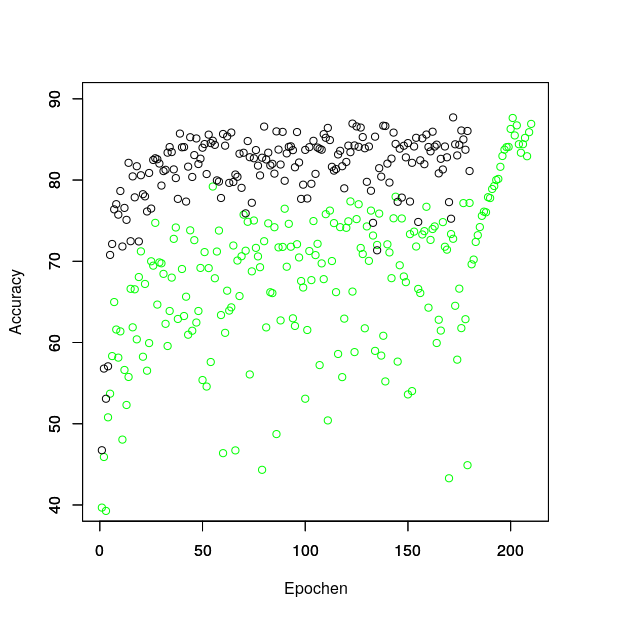
\includegraphics[width=0.47\textwidth]{KapitelPartB/Images/morph6.png}\label{abb:morph6}}
     \hfill
     \subfloat[][]{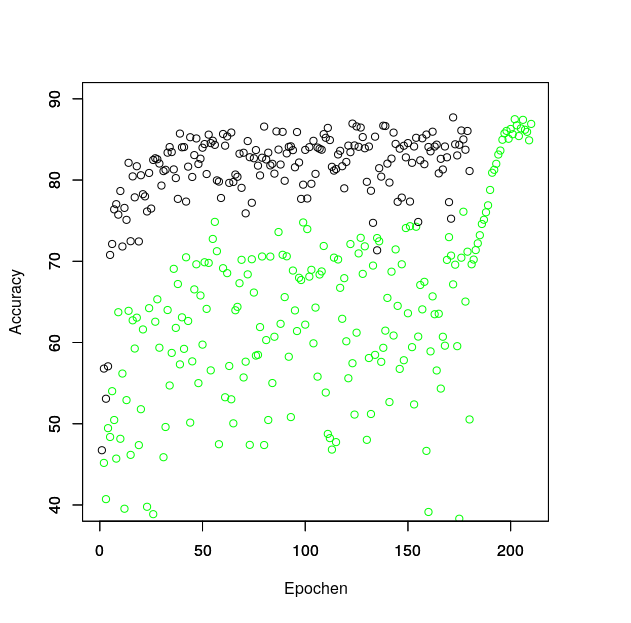
\includegraphics[width=.47\linewidth]{KapitelPartB/Images/morph7.png}\label{abb:morph7}}\\
     \subfloat[][]{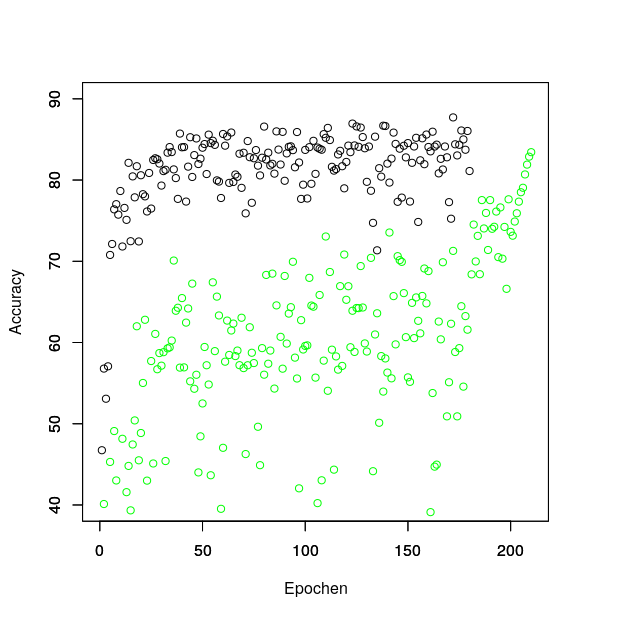
\includegraphics[width=.47\linewidth]{KapitelPartB/Images/morph8.png}\label{abb:morph8}}
     \subfloat[][]{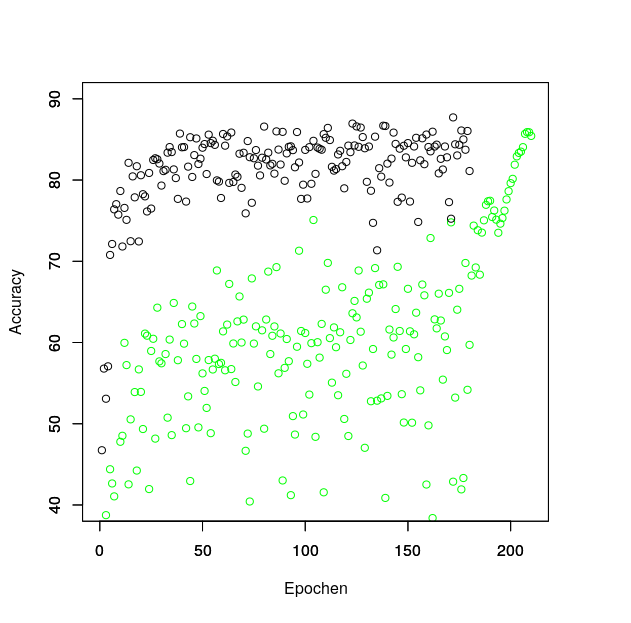
\includegraphics[width=.47\linewidth]{KapitelPartB/Images/morph9.png}\label{abb:morph9}}\\
     \subfloat[][]{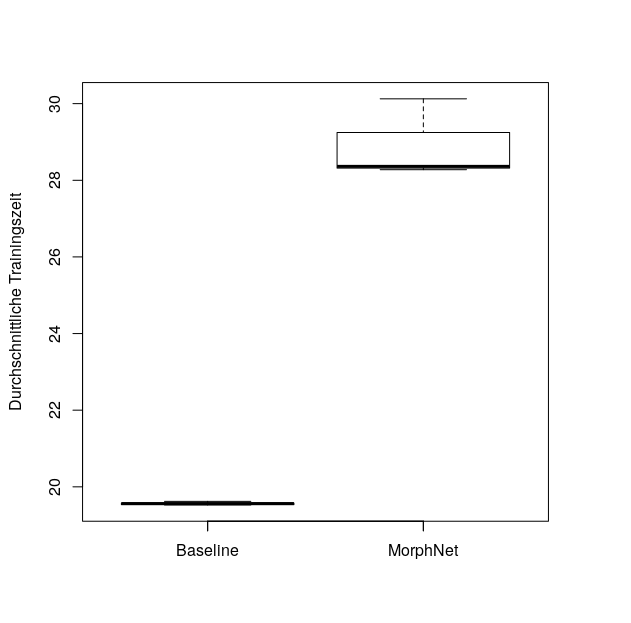
\includegraphics[width=.47\linewidth]{KapitelPartB/Images/morphTime.png}\label{abb:morphTime}}

     \caption{Effekt verschieden großer $\lambda$ auf die Accuracy nach 210 Epochen im Vergleich zum Baseline Netz für (a) $\lambda = 1 \cdot 10^{-8}$ (b) $\lambda = 2 \cdot 10^{-8}$ (c) $\lambda = 3 \cdot 10^{-8}$ (d) $\lambda = 4 \cdot 10^{-8}$. (e) Boxplot zum Vergleich der durchschnittlichen Trainingszeit von Baseline Netz mit dem MorphNet Netz}
     \label{abb:morphAcc}
\end{figure}

Im Gegensatz zur Veröffentlichung kann mit den durchgeführten Experimenten keine Struktur gefunden werden, die besser abschneidet als das Baseline Netz. Möglicherweise ist das Netz hier nach 210 Epochen noch nicht fertig trainiert.
Eine weitere Möglichkeit ist, dass ein besseres Abschneiden des ResNets mit Cifar10 nicht durch eine bessere Struktur mit der Beschränkung der Zielgröße möglich ist. Für diesen Grund spricht, dass mittels Net2Net eine bessere breitere Struktur gefunden wurde, in dem das komplette Baseline Netz mit dem Faktor zwei in der Breite verdoppelt wurde. 

In Abbildung \ref{abb:morphTime} ist zu sehen wie die hier durchgeführten Experimente zeitlich abschneiden.  
Um zu überprüfen, wie groß die Wahrscheinlichkeit für einen Fehler 1. Art ist wird zwischen den durchschnittlichen Trainingszeit des Baseline Netzes und des MorphNet Netzes ein t-Test durchgeführt. Es ergibt sich ein p-Wert von 0.0002. Damit sind die Zeiten des MorphNet Algorithmus hier signifikant höher, als beim Baseline Netz. 









\begin{comment}
\chapter{Additive Verfahren}

\subsection{Zahlenformate}\label{sec:zahlen}
\todo[inline]{Text fertig schreiben; etwa 4 Stunden}
\begin{itemize}
 \item FP16 bereits probiert
\end{itemize}


FP16 nur auf RTX 2080 sinnvoll
Bietet nach erster Messung etwa 28 \% Prozent Gewinn.

Code für dieses Verfahren liegt vor: Amp apex von Nvidia

AMP bietet 3 mögliche Optimierungsstufen:

O1
Patch all Torch functions and Tensor methods to cast their inputs according to a whitelist-blacklist model. Whitelist ops (for example, Tensor Core-friendly ops like GEMMs and convolutions) are performed in FP16. Blacklist ops that benefit from FP32 precision (for example, softmax) are performed in FP32. O1 also uses dynamic loss scaling, unless overridden.

02
casts the model weights to FP16, patches the models forward method to cast input data to FP16, keeps batchnorms in FP32, maintains FP32 master weights, updates the optimizer’s paramgroups so that the optimizer.step() acts directly on the FP32 weights (followed by FP32 master weight-FP16 model weight copies if necessary), and implements dynamic loss scaling (unless overridden). Unlike O1, O2 does not patch Torch functions or Tensor methods.


O3
may not achieve the stability of the true mixed precision options O1 and O2. However, it can be useful to establish a speed baseline for your model, against which the performance of O1 and O2 can be compared. If your model uses batch normalization, to establish speed of light you can try O3 with the additional property override keepBatchnormfp32=True (which enables cudnn batchnorm, as stated earlier).

Hier nur O0, O1 und O2 dargestellt, da O3 absolut nicht mithalten kann was Performance angeht.

\begin{figure}[h]
 \centering
 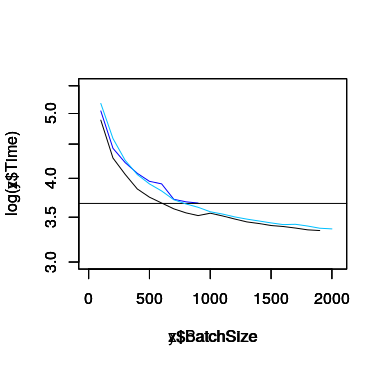
\includegraphics[width=0.8\textwidth]{KapitelPartB/Images/timeVsBatchSize_Amp.png}
 % timeVsBatchSize_Amp.png: 387x367 px, 96dpi, 10.24x9.71 cm, bb=0 0 290 275
 \caption{Vergleich Trainingszeit einer Epoche für verschiedene Optimierungsstufen von Amp Apex. DunkelBlau=O0; Schwarz = O1; Hellblau=O2}
 \label{fig:amp}
\end{figure}
\url{https://developer.download.nvidia.com/video/gputechconf/gtc/2019/presentation/s9998-automatic-mixed-precision-in-pytorch.pdf} zeigt, dass bezüglich der Accuracy kein Verlust zu erwarten ist.

Da O2 gegenüber O1 keinen signifikanten zusätzlichen Gewinn bringt nutze O1.



\subsection{LARS}\label{sec:lars}
\todo[inline]{Experimente fast fertig (3x mal auf einer Graka für 50 min); dann etwa 3 Stunden fürText + Evaluierung}




Es stellt sich die Frage, ob das einen so grossen Einfluss auf die Ausführungszeit hat.



Man sieht, dass mit steigender Batchgröße die Ausführungszeit sinkt. 

Errechne zusätzlich noch ein Modell, wo abhängig von der Modellgrösse währenddem Pruning die Batchgrösse angepasst wird.





\subsection{Beschleunigung der Berechnung des Gradientenabstiegverfahren}
\todo[inline]{ab hier löschen}

Accelerating CNN Training by Sparsifying Activation Gradients funktioniert nur auf Toy-Benchmarks 


\subsubsection{Weight Normalization: A Simple Reparameterization
to Accelerate Training of Deep Neural Networks}


Könnte funktionieren. Code für Lasagne: https://github.com/TimSalimans/weight\_norm


\subsubsection{Accelerating Deep Neural Network Training with Inconsistent Stochastic Gradient Descent}

Interessant bisher kein Code verfügbar

\subsubsection{Accelerated CNN Training Through Gradient Approximation }

Interessant bisher kein Code verfügbar


\end{comment}



\chapter{Evaluation des Beschneidens des Netzes}\label{sec:ptexperimente}
\section{Evaluation bei gleichbleibender Batchgröße}

Die Untersuchung von PruneTrain basiert auf einer bereits vorgefertigten Implementierung \cite{ptImpl}. In dieser Implementierung ist alles bis auf die Anpassung der Batchgröße an das kleiner werdende Netz enthalten. Das Ergebnis der Ausführung von PruneTrain auf der Hardware wird mit den Ergebnissen aus der Veröffentlichung verglichen \cite{prunetrain}. Ziel der Experimente ist es zu evaluieren, wie eine Änderung der verschiedenen Hyperparameter die Trainingszeit und die Accuracy beeinflusst. Im Gegensatz zur Veröffentlichung von PruneTrain wird hier statt auf mehreren GPUs nur auf einer GPU gerechnet. So kann evaluiert werden, wieviel der PruneTrain Effekte auf das Setup mit mehreren GPUs in der Veröffentlichung zurückzuführen sind. 

Bei der Evaluierung der Einflüsse werden die veränderbaren Hyperparameter von PruneTrain einzeln verändert, um den Einfluss der einzelnen Veränderungen zu untersuchen.  
Die veränderbaren Hyperparameter sind:
\begin{itemize}
 \item Lasso-Ratio $0,2$
 \item Rekonfigurationsinterval $5$
 \item Grenzwert $0,0001$
 \item Lernrate $0,1$
\end{itemize}
Hinter den veränderbaren Hyperparameter steht jeweils der Wert, den der Hyperparameter hat, wenn er im aktuellen Experiment nicht verändert wird.
Betrachte eine feste Batchgröße von 256 über 180 Epochen und vergleiche diese mit dem Baseline-Netzes aus Kapitel \ref{sec:baseline}. Für jede Gruppe von Experimenten werden 5 Experimente durchgeführt. 


\subsubsection{Einfluss von verschiedenen Lasso-Ratio Werten auf das Netz}
Die Lasso-Ratio gibt an, wie stark das Netz beschnitten werden soll. In diesen Experimenten wird die Lasso-Ratio von 0,05 bis 0,25 in 0,05er Schritten verändert. In Abbildung \ref{abb:lasso1} ist zusehen, dass mit steigender Lasso-Ratio durchschnittlich weniger Trainingszeit gebraucht wird. Für die durchschnittliche Trainingszeit eines Experiments wird das arithmetische Mittel über alle Epochen angewandt. Die Experimente werden dann nach ihrer Zugehörigkeit einsortiert und als Boxplot in Abbildung \ref{abb:lasso1} dargestellt. Trotz der nachlassenden Trainingszeit mit steigender Lasso-Ratio ist die Trainingszeit des Baseline-Netzes signifikant schneller. Dies ist durch den Overhead erklärbar, welcher durch das Beschneiden des Netzes entsteht.
Um zu überprüfen, wie signifikante diese Unterschiede zwischen den Experimentengruppen hier sind werden paarweise t-Tests mit einem Signifikanzniveau $\alpha=0,05$ durchgeführt. Die resultierenden p-Werte sind in Tabelle \ref{tab:lasso1} zu sehen.

\begin{table}[]
\centering
\begin{tabular}{l|c|c|c|c|c|}
\cline{2-6}
& \multicolumn{1}{l|}{Lasso $0,05$} & \multicolumn{1}{l|}{Lasso $0,1$} & \multicolumn{1}{l|}{Lasso $0,15$} & \multicolumn{1}{l|}{Lasso $0,2$} & \multicolumn{1}{l|}{Lasso $0,25$} \\ \hline
\multicolumn{1}{|l|}{Baseline}                             & $6,9\cdot10^{-6}$   & $<2,2\cdot10^{-16} $   & $<2,2\cdot 10^{-16}$     & $2,9\cdot 10^{-5}$   & $4,9\cdot10^{-5}$    \\ \hline
\multicolumn{1}{|l|}{Lasso $0,05$}                             & X                               & $0,0299$                         & $0,0199$                          & $0,0002$                         & $5,6\cdot 10^{-5}$    \\ \hline
\multicolumn{1}{|l|}{Lasso $0,1$}                             & X                               & X                              & $0,0025$                          & $0,0035$                         & $0,0016$                          \\ \hline
\multicolumn{1}{|l|}{Lasso $0,15$}   & X                               & X                              & X                               & $0,0046$                         & $0,0019$                          \\ \hline
\multicolumn{1}{|l|}{Lasso $0,2$}                             & X                               & X                              & X                               & X                              & \cellcolor[HTML]{FE0000}$0,2540$                          \\ \hline
\end{tabular}
\caption{p-Werte für den t-Tests zu den durchschnittlichen Trainingszeiten der Lasso-Ratio Experimente}
\label{tab:lasso1}
\end{table}
Da bis auf den t-Test zwischen den Lasso Werten 0,2 und 0,25 alle p-Werte kleiner dem Signifikanzniveau sind ist ein Fehler 1.Art sehr unwahrscheinlich. Daher lässt sich für die übrigen Wertepaare die Aussage treffen, dass sie einen statistisch signifikanten Unterschied der Mittelwerte haben. Somit entsteht durch das Erhöhen der Lasso-Ratio ein signifikante Einsparung an Trainingzeit gegenüber einer kleineren Lasso-Ratio. Gegenüber den durchschnittlichen Trainingszeiten des Baseline-Netzes ist allerdings das Baseline in allen Fällen signifikante schneller.  


In Abbildung \ref{abb:lasso2} ist die Accuracy der verschiedenen Experimente abgebildet. Es fällt auf, dass das Baseline-Netz im Mittel etwas besser ausfällt als die Experimente mit dem Lasso-Ratio 0,05.
\begin{figure}
     \centering
     \subfloat[][]{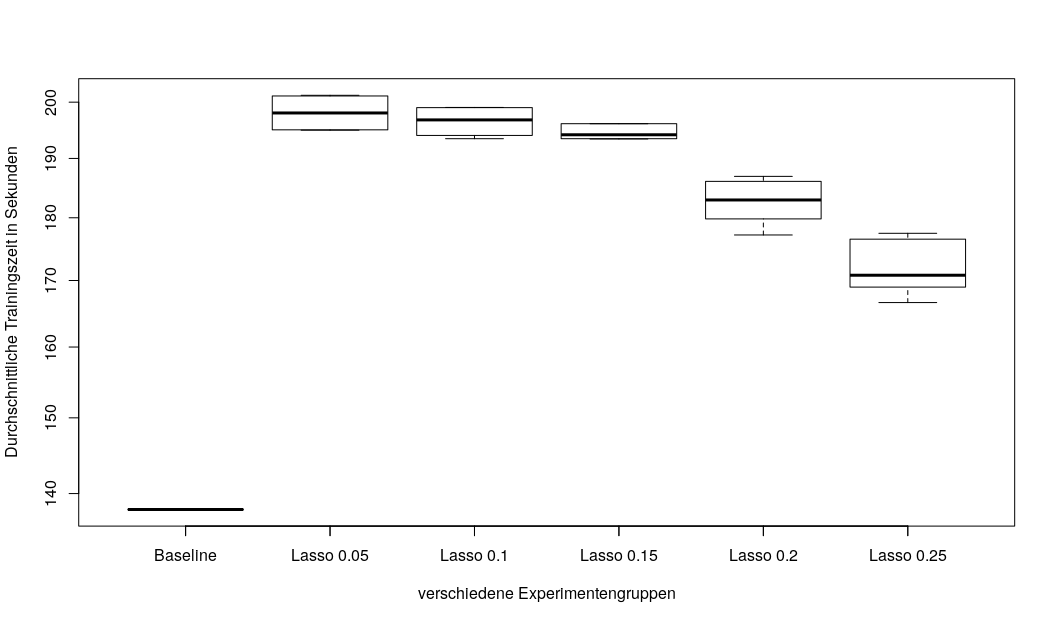
\includegraphics[width= .5\linewidth]{KapitelPartB/Images/lasso1.png}\label{abb:lasso1}}
     \hfill
     \subfloat[][]{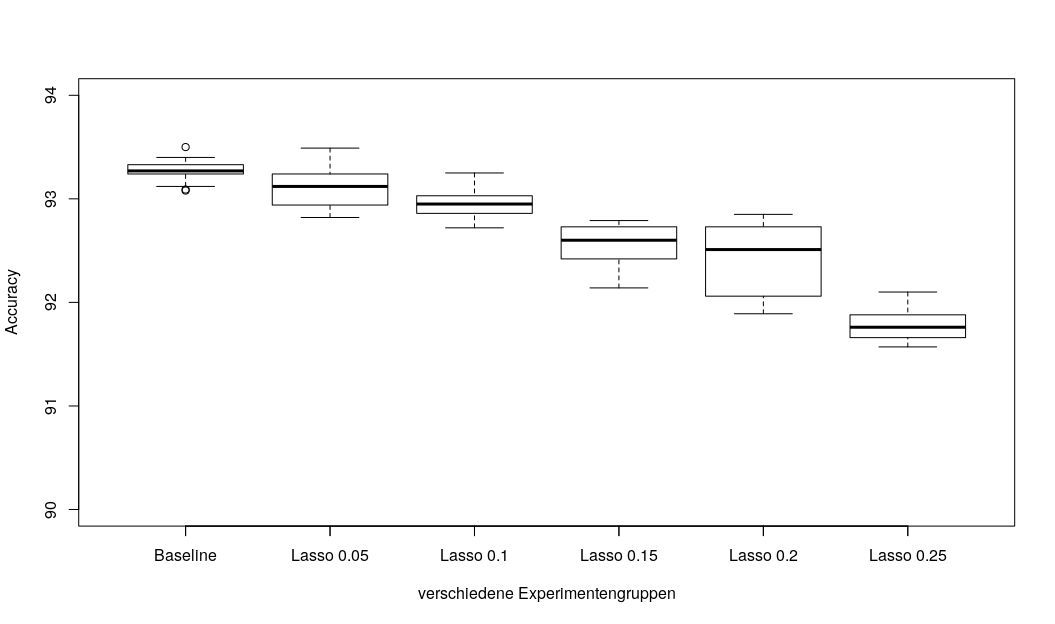
\includegraphics[width=.5\linewidth]{KapitelPartB/Images/lasso2.png}\label{abb:lasso2}}
     \caption{Lasso-Ratio Experiment: (a) Boxplot der durchschnittlichen Trainingszeit (b) Boxplot der Accuracy}
     \label{abb:lasso}
\end{figure}
In Tabelle \ref{tab:lasso2} sind die Werte für den paarweisen t-Test zwischen den Accuracy der Experimentegruppen abgebildet. Das Signifikanzniveau beträgt $\alpha =0,05$. In der Tabelle ist zu sehen, dass die rot hinterlegten p-Werte größer als das Signifikanzniveau sind. Somit ist für diese paarweisen Accuracy die Wahrscheinlichkeit für einen Fehler 1. Art zu groß für die Aussage, dass die Accuracy der Experimente einen unterschiedlichen Mittelwert haben. Es lässt sich jedoch erkennen, dass für jede Zeile die p-Werte kleiner werden, je größer die Lasso-Ratio wird. Somit lässt sich die begründete Aussage treffen, dass mit steigender Lasso-Ratio die Accuracy signifikant abnimmt.
Die fehlende Signifikanz dieser Paare kann sowohl an der fehlenden statistischen Signifikanz liegen als auch an der kleinen Anzahl an Experimenten pro Gruppe. Da die hier getroffene Aussage allerdings ausreicht wird das Experiment nicht mit grösserer Anzahl wiederholt.




\begin{table}[]
\caption{p-Werte für den t-Tests zu den Accuracy-Werten der Lasso-Ratio Experimente}
\centering
\begin{tabular}{l|c|c|c|c|c|}
\cline{2-6}
                                & \multicolumn{1}{l|}{Lasso $0,05$} & \multicolumn{1}{l|}{Lasso $0,1$} & \multicolumn{1}{l|}{Lasso $0,15$} & \multicolumn{1}{l|}{Lasso $0,2$} & \multicolumn{1}{l|}{Lasso $0,25$} \\ \hline
\multicolumn{1}{|l|}{Baseline}   & \cellcolor[HTML]{FE0000}$0,7068$  & \cellcolor[HTML]{FE0000}$0,4952$ & \cellcolor[HTML]{FE0000}$0,2586$  & $0,0018$                         & $8,6\cdot 10^{-6}$     \\ \hline
\multicolumn{1}{|l|}{Lasso $0,05$}& X                               & \cellcolor[HTML]{FE0000}$0,2898$ & \cellcolor[HTML]{FE0000}$0,1341$  & $0,0010$                       & $1,0\cdot 10^{-7}$    \\ \hline
\multicolumn{1}{|l|}{Lasso $0,1$} & X                               & X                              & \cellcolor[HTML]{FE0000}$0,6530$   & $0,0041$         ig              & $7,5\cdot10^{-5}$    \\ \hline
\multicolumn{1}{|l|}{Lasso $0,15$}& X                               & X                              & X                               & $0,0072$                       & $0,0001$                       \\ \hline
\multicolumn{1}{|l|}{Lasso $0,2$} & X                               & X                              & X                               & X                              & $0,0182$                         \\ \hline
\end{tabular}
\label{tab:lasso2}
\end{table}



\subsubsection{Experimente zum Rekonfigurationsintervall}
 Als nächste Größe wird der Einfluss des Rekonfigurationsintervalls überprüft. Die entsprechenden Grafiken sind in Abbildung \ref{abb:reconf} zu sehen. In Abbildung \ref{abb:reconf1} sind für die verschiedenen Experimente die Trainingszeiten pro Epoche zu sehen. Dabei werden drei verschiedene Rekonfigurationsintervalle (2,5 und 10) verglichen. In Abbildung \ref{abb:reconf1} lässt sich für die verschiedenen durchschnittlichen Trainingszeiten der Experimente zum Rekonfigurationsintervall kaum Unterschiede erkennen. Daher ist in Abbildung \ref{abb:reconf2} ein Boxplot ohne die Baseline Werte abgebildet. Der Grund hierfür ist, dass sich die Zeitersparnis durch das vermehrte Beschneiden aufgrund einem kleinerem Rekonfigurationsintervall mit dem nötigen Overhead der häufigeren Rekonfiguration aufhebt.
 
 
 In Tabelle \ref{tab:reconf} ist bestätigt, das zwischen den durchschnittlichen Trainingszeiten der Experimente kein signifikanter Unterschied ist. Dabei ist zu bedenken, dass die Experimentanzahl mit fünf relativ klein ist. Wichtiger als die hier eventuell minimale Einsparung von Trainingszeit ist die Auswirkung auf die Accuracy.
 


\begin{table}[]
\caption{p-Werte für den t-Tests zu den durchschnittlichen Trainingszeiten der Rekonfigurationsinterval Experimente }
\centering
\begin{tabular}{l|c|c|c|}
\cline{2-4}
                                & \multicolumn{1}{l|}{Rekonf 2}     & \multicolumn{1}{l|}{Rekonf 5}     & \multicolumn{1}{l|}{Rekonf 10}    \\ \hline
\multicolumn{1}{|l|}{Baseline}  & \cellcolor[HTML]{FFFFFF}$4,7\cdot 10^{-7}$ & \cellcolor[HTML]{FFFFFF}$6,4\cdot 10^{-5}$ & \cellcolor[HTML]{FFFFFF}$0.0002$ \\ \hline
\multicolumn{1}{|l|}{Rekonf 2}  & X                                 & \cellcolor[HTML]{FE0000}$0.6034$    & \cellcolor[HTML]{FE0000}$0.9853$    \\ \hline
\multicolumn{1}{|l|}{Rekonf 5}  & X                                 & X                                 & \cellcolor[HTML]{FE0000}$0.9859$    \\ \hline
\end{tabular}
\label{tab:reconf}
\end{table}
 
\begin{figure}
     \centering
     \subfloat[][]{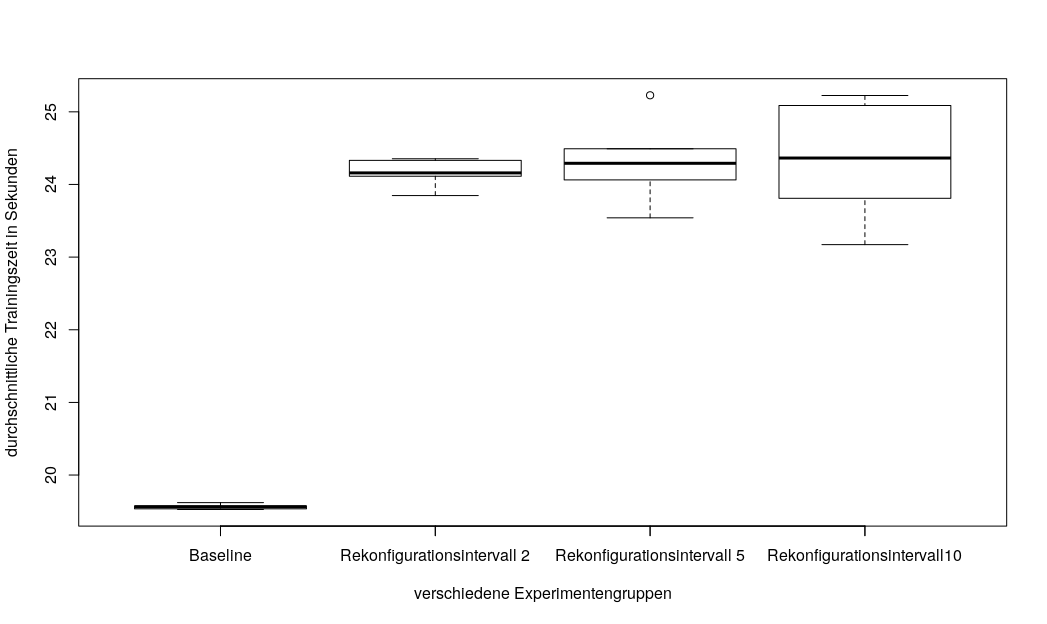
\includegraphics[width= .45\textwidth]{KapitelPartB/Images/reconf1.png}\label{abb:reconf1}}
     \hfill
     \subfloat[][]{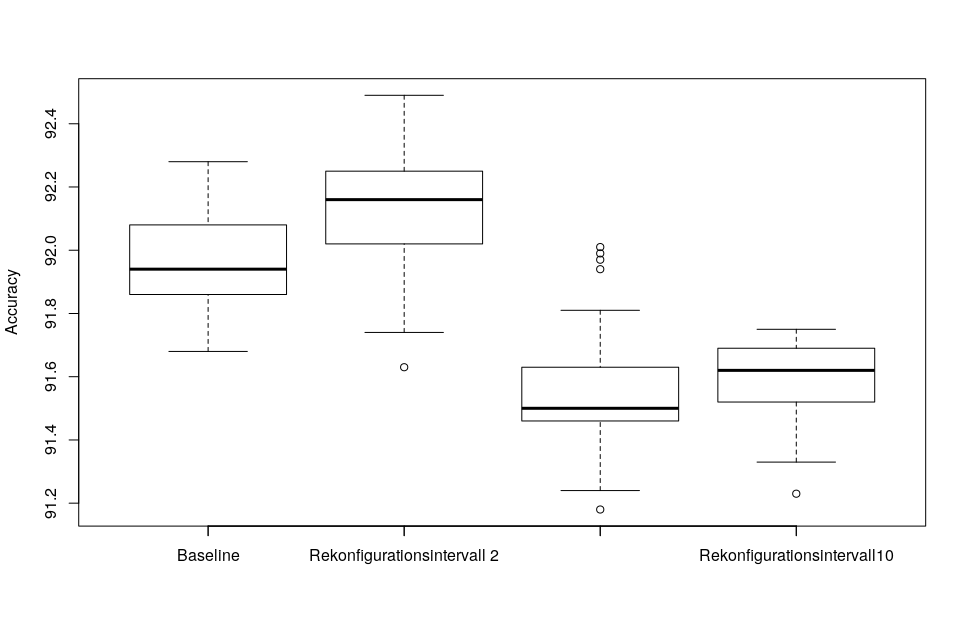
\includegraphics[width= .45\textwidth]{KapitelPartB/Images/reconf2.png}\label{abb:reconf2}}
     \\
     \subfloat[][]{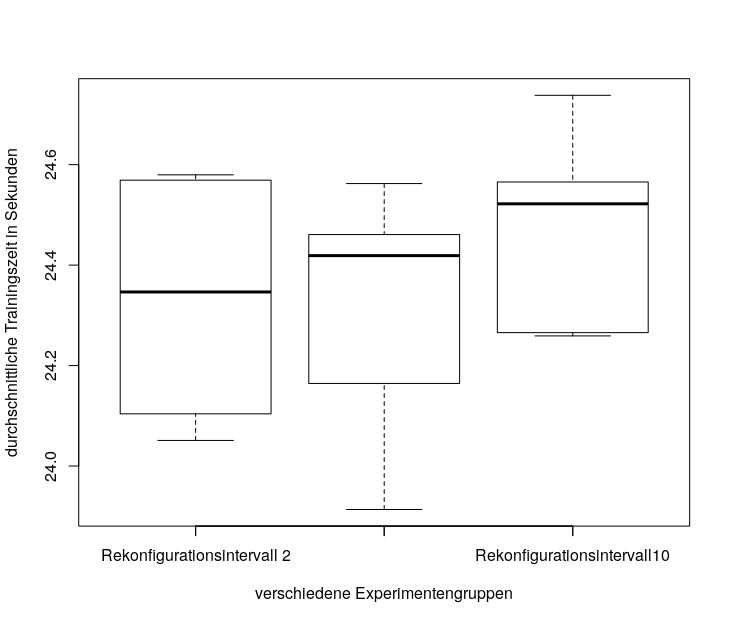
\includegraphics[width=.45\textwidth]{KapitelPartB/Images/reconf3.png}\label{abb:reconf3}}
     \caption{Experimente zum Rekonfigurationsintervall: (a) Boxplot der durchschnittlichen Trainingszeit (b) Boxplot der durchschnittlichen Trainingszeit ohne Baseline-Netz (c) Boxplot der Accuracy}
     \label{abb:reconf}
\end{figure}

In Abbildung \ref{abb:reconf3} ist zu sehen, wie sich die Accuracy bei diesen Experimenten verhält. Zu sehen ist, dass die Accuracy keine klare Tendenz hat. Dies zeigt sich auch in den t-Test in Tabelle \ref{tab:reconf2}. Hier ist die Anzahl an Experimenten wohl zu gering, um eine klare Aussage zu treffen. Da die Unterschiede hier aber so gering sind ist die Wahl des Rekonfigurationsintervall nicht so wichtig.


\begin{table}[]
\caption{p-Werte für den t-Tests zu den Accuracys der Rekonfigurationsinterval Experimente}
\begin{tabular}{l|c|c|c|c|}
\cline{2-5}
                                & \multicolumn{1}{l|}{Baseline} & \multicolumn{1}{l|}{Rekonf 2}  & \multicolumn{1}{l|}{Rekonf 5}  & \multicolumn{1}{l|}{Rekonf 10} \\ \hline
\multicolumn{1}{|l|}{Baseline}  & X                             & \cellcolor[HTML]{FFFFFF}0.0478 & \cellcolor[HTML]{FE0000}0.1111 & \cellcolor[HTML]{FFFFFF}0.0105 \\ \hline
\multicolumn{1}{|l|}{Rekonf 2}  & X                             & X                              & \cellcolor[HTML]{FE0000}0.43   & \cellcolor[HTML]{FE0000}0.1824 \\ \hline
\multicolumn{1}{|l|}{Rekonf 5}  & X                             & X                              & X                              & \cellcolor[HTML]{FE0000}0.9938 \\ \hline
\multicolumn{1}{|l|}{Rekonf 10} & X                             & X                              & X                              & X                              \\ \hline
\end{tabular}
\label{tab:reconf2}
\end{table}
 
  
\subsubsection{Experimente zur Lernrate}
\todo[inline]{Vergleich mit Baseline und verschiedenen LR}
Der Einfluss der Lernrate auf das Beschneiden des Netzes wird mit fünf verschiedenen Lernraten untersucht. Beginnend mit der Lernrate $0,2$ und für jede weitere der fünf Lernraten die Hälfte der vorherigen.
Die durchschnittliche Trainingszeit in Sekunden für verschiedene Lernrate ist in Abbildung \ref{abb:lr} zu sehen. Es ist deutlich zu sehen, dass mit sinkender Lernrate die Trainingszeit steigt. Das bedeutet, dass mit sinkender Lernrate weniger von Netz beschnitten wird, dies sorgt allerdings nicht zu einem verringerten Overhead. Der Overhead hängt bei diesem Verfahren von der Häufigkeit der Rekonfiguration ab.


In Tabelle \ref{tab:lr1} sind die p-Werte für die paarweisen t-Test zu sehen, die berechnen wie wahrscheinlich es ist, dass ein Fehler 1. Art auftritt. Da die p-Werte bis auf einen Wert unter dem Signifikanzniveau von $\alpha = 0,05$ ist die hier getroffene Aussage statistisch belegt.


\begin{table}[]
\caption{p-Werte für den t-Tests zu den Accuracys der durchschnittlichen Experimenten zur Lernrate}
\begin{tabular}{l|c|c|c|c|l|}
\cline{2-6}
                               & \multicolumn{1}{l|}{Baseline} & \multicolumn{1}{l|}{LR 0,2} & \multicolumn{1}{l|}{LR 0,1}                       & \multicolumn{1}{l|}{LR 0,05} & LR 0,025                       \\ \hline
\multicolumn{1}{|l|}{Baseline} & X                             & 0,0003                      & \multicolumn{1}{l|}{5,265*10\textasciicircum{}-5} & \multicolumn{1}{l|}{0,0003}  & 4,888*10\textasciicircum{}-6   \\ \hline
\multicolumn{1}{|l|}{LR 0,2}   & X                             & X                           & 0,0001                                            & 0,0011                       & 9,211*10\textasciicircum{}-7   \\ \hline
\multicolumn{1}{|l|}{LR 0,1}   & X                             & X                           & X                                                 & 0,0332                       & 0.0011                         \\ \hline
\multicolumn{1}{|l|}{LR 0,05}  & X                             & X                           & X                                                 & X                            & \cellcolor[HTML]{FE0000}0,9074 \\ \hline
\multicolumn{1}{|l|}{LR 0,025} & X                             & X                           & X                                                 & X                            & \multicolumn{1}{c|}{X}         \\ \hline
\end{tabular}
\label{tab:lr1}
\end{table}
 
 \begin{figure}
     \centering
     \subfloat[][]{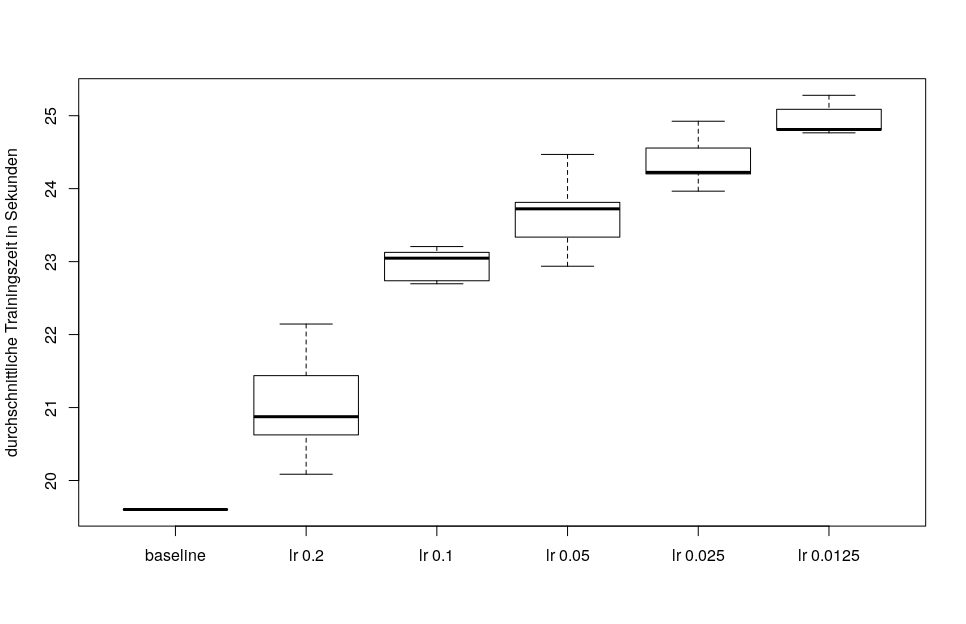
\includegraphics[width= .45\textwidth]{KapitelPartB/Images/lr1.png}\label{abb:lr1}}
     \hfill
     \subfloat[][]{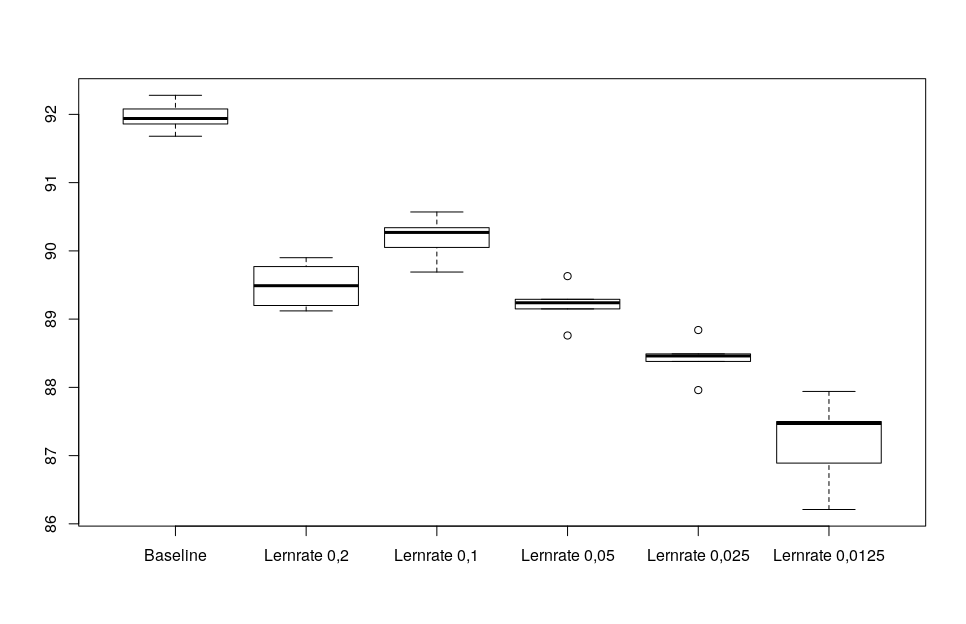
\includegraphics[width= .45\textwidth]{KapitelPartB/Images/lr2.png}\label{abb:lr2}}
     \caption{Experimente zur Lernrate: (a) Boxplot der durchschnittlichen Trainingszeit (b) Boxplot der durchschnittlichen Trainingszeit ohne Baseline-Netz (c) Boxplot der Accuracys}
     \label{abb:lr}
\end{figure}

 In Abbildung \ref{abb:lr2} sind die Accuracy der verschiedenen Lernraten abgildet. Die Lernrate $0.1$ schneidet hier am Besten ab. Dies kann darauf zurück geführt werden, dass bei einer größeren Lernrate weniger Minima in der Verlustfunktion gefunden werden können. Der Effekt bei wesentlich kleineren Lernraten ist, dass der Trainingsprozess zwar mit jedem Schritt in die Richtung des Minimums geht, dabei aber durch die kleine Lernrate das tatsächliche Minimum innerhalb der 180 Epochen nicht erreicht wird oder mit der kleinen Lernrate ein lokales Minimum nicht verlassen werden kann. In Tabelle \ref{tab:lr2} sind die p-Werte der paarweisen t-Tests zu sehen. Bis auf zwei Werte sind diese kleiner als das Signifikanzniveau $\alpha=0,05$. Damit ist die Wahrscheinlichkeit für einen Fehler 1.Art bis auf diese zwei Werte kleiner als 5 \%. Damit sind die hier getroffenen Aussagen statistisch belegt sind.
 
\begin{table}[]
\caption{p-Werte für den t-Tests zu den Accuracys der Experimente zu den Lernraten}
\begin{tabular}{l|c|c|c|c|l|}
\cline{2-6}
                               & \multicolumn{1}{l|}{Baseline} & \multicolumn{1}{l|}{LR 0,2}  & \multicolumn{1}{l|}{LR 0,1} & \multicolumn{1}{l|}{LR 0,05}                        & LR 0,025                       \\ \hline
\multicolumn{1}{|l|}{Baseline} & X                             & 3,355*10\textasciicircum{}-5 & \multicolumn{1}{l|}{0,0005} & \multicolumn{1}{l|}{\cellcolor[HTML]{FE0000}0,7253} & 0,004                          \\ \hline
\multicolumn{1}{|l|}{LR 0,2}   & X                             & X                            & 0,0003                      & 4,83*10\textasciicircum{}-5                         & 0,0005                         \\ \hline
\multicolumn{1}{|l|}{LR 0,1}   & X                             & X                            & X                           & 0,0006                                              & \cellcolor[HTML]{FE0000}0,8715 \\ \hline
\multicolumn{1}{|l|}{LR 0,05}  & X                             & X                            & X                           & X                                                   & 0,0003                         \\ \hline
\multicolumn{1}{|l|}{LR 0,025} & X                             & X                            & X                           & X                                                   & \multicolumn{1}{c|}{X}         \\ \hline
\end{tabular}
\label{tab:lr2}
\end{table}
 
\subsubsection{Experimente zum Grenzwert}

Der Einfluss des gewählten Thresholds wird hier untersucht. In Abbildung \ref{abb:thres1} sind die durchschnittlichen Trainingszeiten abgebildet. Auch hier ist zu sehen, dass die durchschnittliche Trainingszeit durch die Anwendung des PruneTrain Algorithmus zunimmt.Unter einem bestimmten Threshold-Wert sind hier die durchschnittlichen Trainingszeiten nicht mehr unterscheidbar. In Tabelle \ref{tab:thres1} sind die p-Werte des t-Tests abgebildet, der untersuchen soll wo ein statistisch signifikanter Unterschied zwischen den durchschnittlichen Trainingszeiten der Experimentengruppen herrscht. Die p-Werte stützen die Aussagen.

\begin{table}[]
\caption{p-Werte für den t-Tests zu den durchschnittlichen Trainingszeiten der Experimente zum Threshold}
\begin{tabular}{l|c|c|c|c|l|}
\cline{2-6}
                                       & \multicolumn{1}{l|}{Baseline} & \multicolumn{1}{l|}{Thres. 0,1} & \multicolumn{1}{l|}{Thres. 0,01} & \multicolumn{1}{l|}{Thres. 0,001} & Thres. 0,0001               \\ \hline
\multicolumn{1}{|l|}{Baseline}         & X                             & 0.0003                             & 0.0002                              & 1.778e-05                            & 0.0002                         \\ \hline
\multicolumn{1}{|l|}{Thres. 0,1}    & X                             & X                                  & \cellcolor[HTML]{FE0000}0.0577      & 0.0018                               & 0.0479                         \\ \hline
\multicolumn{1}{|l|}{Thres. 0,01}   & X                             & X                                  & X                                   & \cellcolor[HTML]{FE0000}0.1209       & \cellcolor[HTML]{FE0000}0.9159 \\ \hline
\multicolumn{1}{|l|}{Thres. 0,001}  & X                             & X                                  & X                                   & X                                    & \cellcolor[HTML]{FE0000}0.1450 \\ \hline
\multicolumn{1}{|l|}{Thres. 0,0001} & X                             & X                                  & X                                   & X                                    & \multicolumn{1}{c|}{X}         \\ \hline
\end{tabular}
\label{tab:thres1}
\end{table}


 \begin{figure}
     \centering
     \subfloat[][]{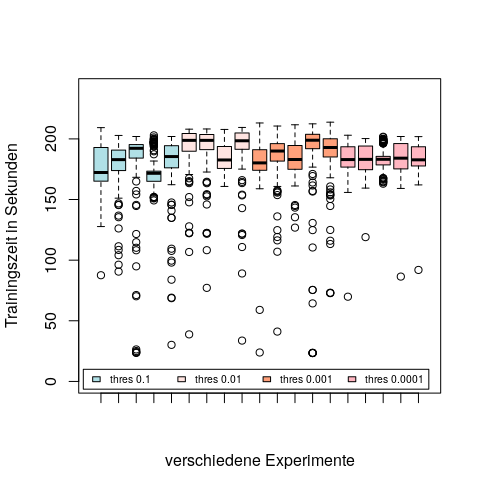
\includegraphics[width= .45\textwidth]{KapitelPartB/Images/thres1.png}\label{abb:thres1}}
     \hfill
     \subfloat[][]{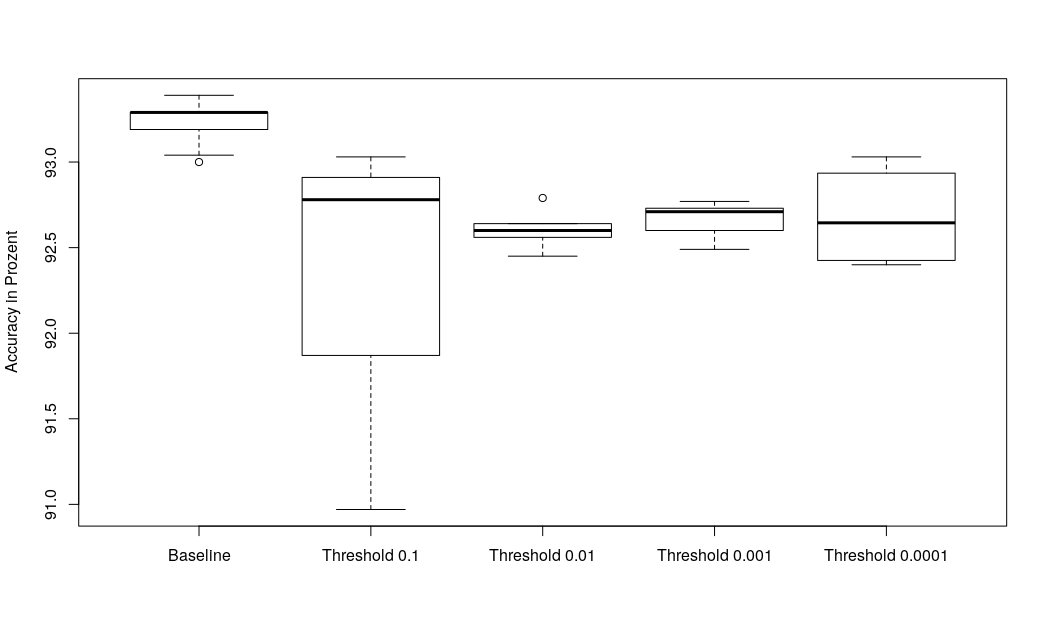
\includegraphics[width= .45\textwidth]{KapitelPartB/Images/thres2.png}\label{abb:thres2}}
     \caption{Experimente zur Threshold: (a) Boxplot der durchschnittlichen Trainingszeit (b) Boxplot der durchschnittlichen Trainingszeit ohne Baseline-Netz (c) Boxplot der Accuracys}
     \label{abb:lr}
\end{figure}
In Abbildung \ref{abb:thres2} ist die Accuracy zu sehen. Aus dieser Abbildung lässt sich keine Tendenz erkennen. Diese Aussage wird durch die p-Werte der paarweisen t-Tests in Tabelle \ref{tab:thres2} gestützt.
 \begin{table}[]
\caption{p-Werte für den t-Tests zu den Accuracys der Experimente zum Threshold}
\begin{tabular}{l|c|c|c|c|l|}
\cline{2-6}
                                     & \multicolumn{1}{l|}{Baseline} & \multicolumn{1}{l|}{Thres. 0,01} & \multicolumn{1}{l|}{Thres. 0,001} & \multicolumn{1}{l|}{Thres. 0,0001} & Thres. 0,00001                 \\ \hline
\multicolumn{1}{|l|}{Baseline}       & X                             & 0,1927                           & \multicolumn{1}{l|}{0,0002}       & \multicolumn{1}{l|}{0,0003}        & 0,0360                         \\ \hline
\multicolumn{1}{|l|}{Thres. 0,01}    & X                             & X                                & \cellcolor[HTML]{FE0000}0,6799    & \cellcolor[HTML]{FE0000}0,6121     & \cellcolor[HTML]{FE0000}0,5968 \\ \hline
\multicolumn{1}{|l|}{Thres. 0,001}   & X                             & X                                & X                                 & \cellcolor[HTML]{FE0000}0,5096     & \cellcolor[HTML]{FE0000}0,6815 \\ \hline
\multicolumn{1}{|l|}{Thres. 0,0001}  & X                             & X                                & X                                 & X                                  & \cellcolor[HTML]{FE0000}0,9076 \\ \hline
\multicolumn{1}{|l|}{Thres. 0,00001} & X                             & X                                & X                                 & X                                  & \multicolumn{1}{c|}{X}         \\ \hline
\end{tabular}
\label{tab:thres2}
\end{table}
\subsubsection{Diskussion der Methode}

Für die Evaluation des Beschneiden des Netzes werden in der Original-Veröffentlichung mehrere GPUs verwendet \cite{prunetrain}. Dies führt dazu, dass bereits in diesem Teil der Implementierung Trainingszeit durch verminderte Kommunikation zwischen den GPUs gespart wird. Da hier nur mit einer GPU evaluiert wird ergibt sich hier noch keine direkte Einsparung an Trainingszeit. Eine weitere Möglichkeit Trainingszeit zu sparen ergibt sich durch Erhöhen der Batchgröße bei kleiner werdendem Netz. Zu beachten ist hier, dass die Speicherauslastung gleich bleiben sollte und eine Vergleichbarkeit mit der Veröffentlichung zu gewährleisten. Diese Evaluierung wird in Kapitel \ref{sec:ptnew} durchgeführt.


\section{Experimente zur Anpassung der Batchgröße beim Beschneiden des Netzes}\label{sec:ptnew}

Die Anpassung der Batchgröße des Netzwerks in der Veröffentlichung arbeitet mit einer Grenze bis zu dieser der Speicher ausgelastet werden darf. 

Die Berechnung der maximalen Batchgröße für eine gegegebene Speichergrösse und Netzarchitektur wird in Kapitel \ref{sec:batch} beschrieben.

\subsection{Berechnung der Batchgröße abhängig vom Speicherverbrauch}\label{sec:batch}
Da sich in Pytorch der freie Speicher nicht direkt auslesen lässt wird mit Hilfe von Experimenten, die auf der GPU durchgeführt werden gemessen wie sich die Speicherauslastung verhält. In Abbildung \ref{abb:memory1} ist zu sehen, wie sich die Speicherauslastung proportional zur Batchgröße verhält. Es ist gut zu erkennen, dass der Zusammenhang linear ist. Die Passgenauigkeit dieses Zusammenhangs kann mittels einer linearen Regression bestimmt werden.  Daher wird mit der roten Gerade eine lineare Regression berechnet. Der maximale Abstand der gemessenen Punkte zur Gerade ist $0,19$ für Punkte, die unter der Gerade liegen sowie $0,67$ für Punkte die über der Gerade liegen. Zusammen mit der graphischen Übereinstimmung ergibt sich klar ein linearer Zusammenhang mit kleinen Abweichungen.
 \begin{figure}
     \centering
     \subfloat[][]{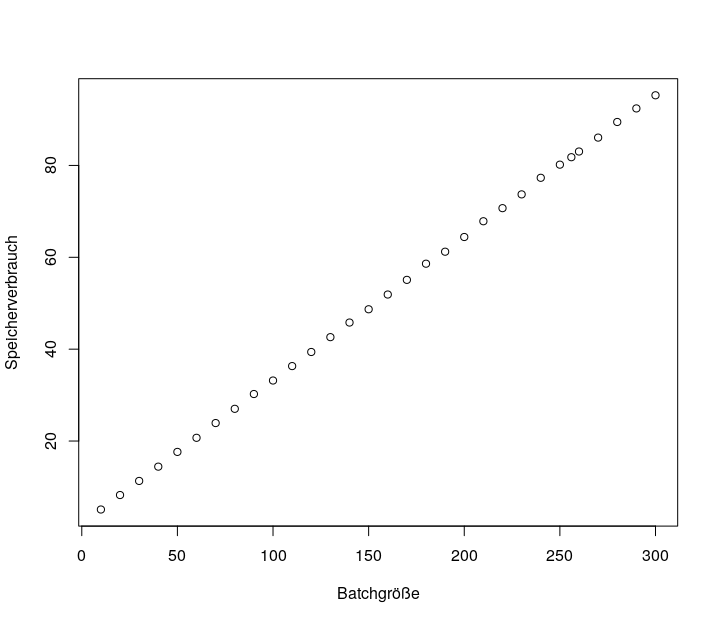
\includegraphics[width= .47\textwidth]{KapitelPartB/Images/memory1.png}\label{abb:memory1}}
     \hfill
     \subfloat[][]{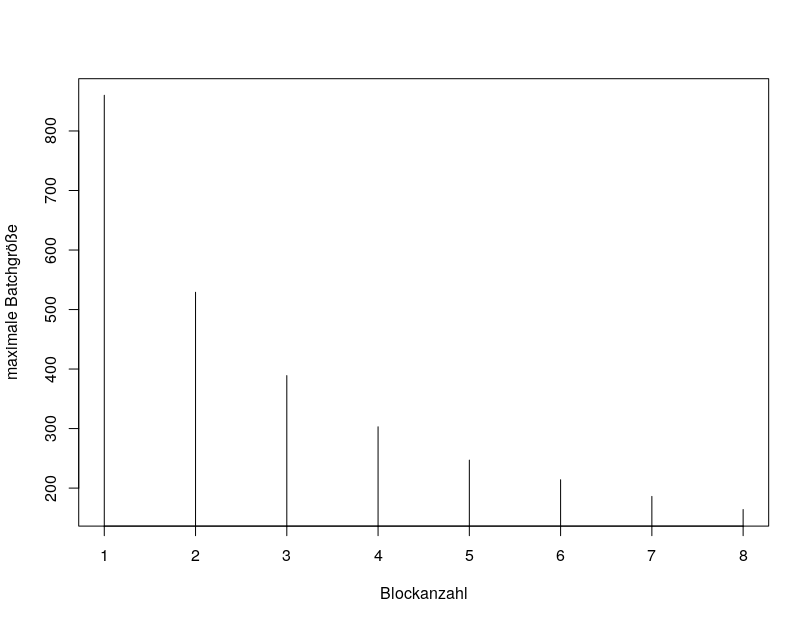
\includegraphics[width= .47\textwidth]{KapitelPartB/Images/memory2.png}\label{abb:memory2}}\\
     \subfloat[][]{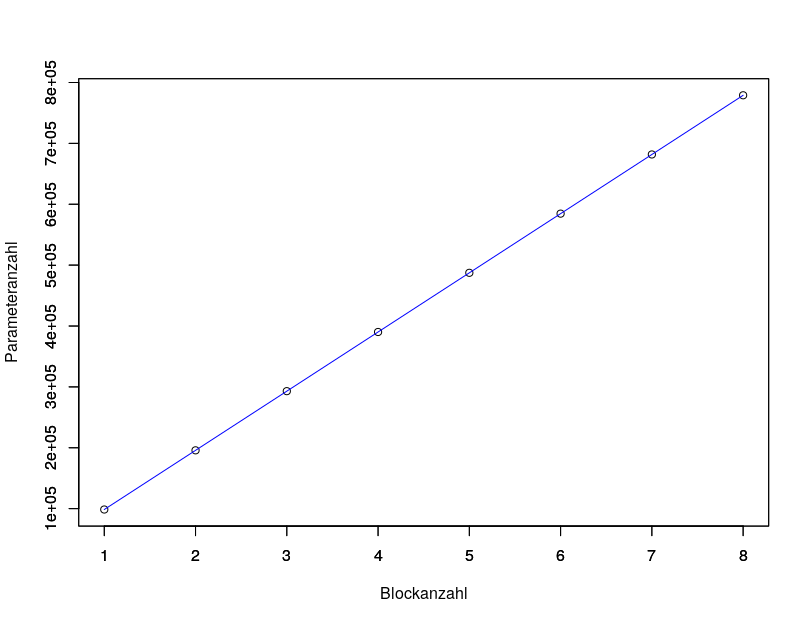
\includegraphics[width= .47\textwidth]{KapitelPartB/Images/memory3.png}\label{abb:memory3}}
     \hfill
     \subfloat[][]{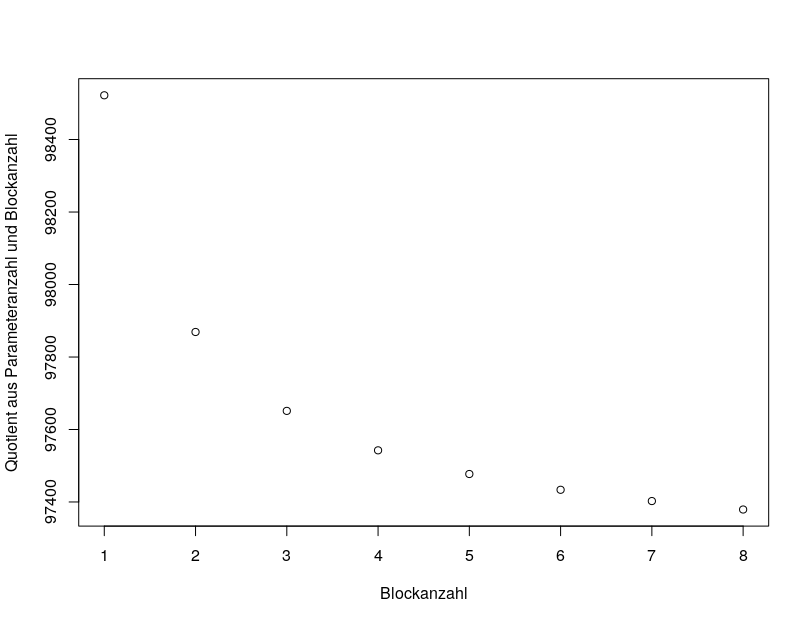
\includegraphics[width= .47\textwidth]{KapitelPartB/Images/memory4.png}\label{abb:memory4}}\\
     \subfloat[][]{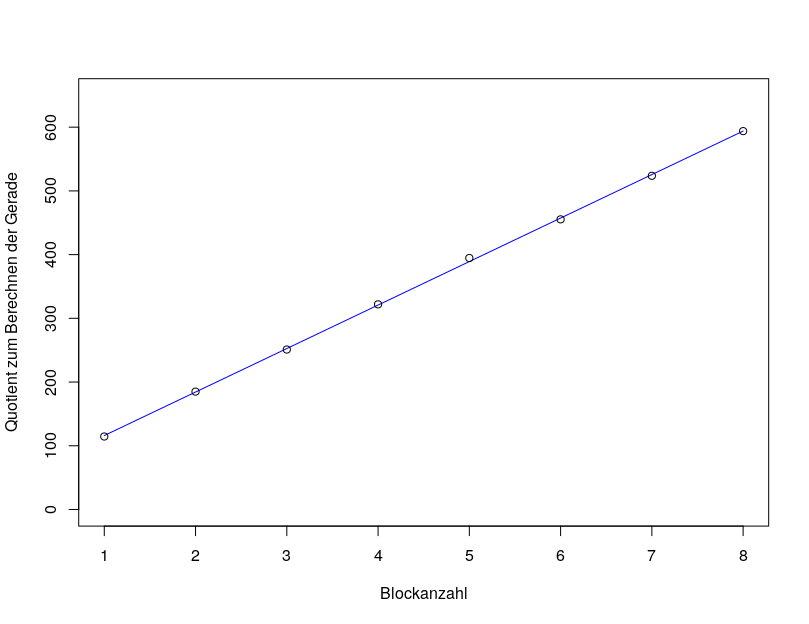
\includegraphics[width= .47\textwidth]{KapitelPartB/Images/memory5.png}\label{abb:memory5}}\\
          
     \caption{Darstellung des Berechnen der Geraden}
     \label{abb:memory}
\end{figure}
Durch diesen linearen Zusammenhang reicht es ein Modell zu bilden, welches für einen Wert des Speicherverbrauchs abhängig von der Netzarchitektur berechnet, wie groß die Batchgröße maximal sein darf. Zu diesem Zweck wird ein Netz mit drei Phasen betrachtet und ein Modell entwickelt mit dem sich die maximale Batchgröße berechnen lässt. Die maximale Batchgröße hängt ab von:

\begin{itemize}
 \item der Blockanzahl
 \item der Phasenanzahl und
 \item der Anzahl an Schichten pro Block
 \item Breite der Schichten je Phase
\end{itemize}
In Abbildung \ref{abb:memory2} ist abgebildet, wie sich die Blockanzahl bei gleichbleibender Speicherauslastung auf die maximale Batchgröße auswirkt. Die Blockanzahl wirkt sich wie zu sehen ist nicht linear auf die maximale Batchgröße aus. Die maximale Blockanzahl hängt ab von der maximalen Speicherauslastung während einer Epoche. Dies ist abhängig von der Blockgröße, da aufgrund der Kurzschlussverbindungen die Ausgabe jedes Blocks zwischengespeichert werden muss.
Betrachtet man hingegen den Zusammenhang zwischen Blockanzahl und Parameteranzahl, wie in Abbildung \ref{abb:memory3} abgebildet, so ergibt sich hier ein linearer Zusammenhang. In Abbildung \ref{abb:memory4} ist der Zusammenhang zwischen Blockanzahl und dem Quotienten aus Parameteranzahl und Blockanzahl zu sehen. Der Verlauf dieser Kurve ähnelt dem Verlauf von Abbildung \ref{abb:memory2}. In Abbildung \ref{abb:memory5} wird daher der Quotient aus diesen beiden Größen gegen die Blockanzahl abgebildet und eine Gerade mit linearer Regression berechnet.


Um die Wahrscheinlichkeit zu prüfen, dass in Abbildung \ref{abb:memory} fälschlicher Weise ein linearer Zusammenhang angenommen wird, wird ein t-Test ausgeführt.
Es ergibt sich die Alternativ- und Nullhypothese:
\begin{align*}
 H_0: \text{Es besteht kein linearer Zusammenhang zwischen dem Quotienten } G \\
 \text{und der Anzahl von Blöcken} \\
 H_1: \text{Es besteht ein linearer Zusammenhang zwischen dem Quotienten } G \\ 
 \text{ und der Anzahl von Blöcken}
\end{align*}
Mit einem Signifikanzniveau von $\alpha =0,05$ und einem $p$-Wert von $p=3,824 \cdot 10^{-12}$ ist die Nullhypothese abzulehnen, und die Alternativhypothese anzunehmen. 

Mit Hilfe dieses linearen Zusammenhangs lässt sich bei gegebener Parameteranzahl $(PA)$ und Blockanzahl $(BA)$ die maximale Batchgröße $(BG)$ berechnen:

\begin{equation}
 BG=\frac{PA}{BA\left( 68,25 \cdot BA + 47,85\right)}
\end{equation}


Da einzelne Punkte einen maximalen Abstand von $d=2,07$ zur Geraden wurde das Ergebnis durch Multiplikation mit $0,98$ ein Sicherheitsabstand eingeführt.


\subsection{Evaluierung der Anpassung der Batchgröße an die Netzgröße}

Da sich für ein gegebenes Netz die Speicherauslastung abhängig von der Batchgröße ein linearer Zusammenhang ergibt, kann die Batchgröße direkt angepasst werden, sobald das beschnittene Netz für eine Epoche trainiert hat. Es wird per Dreisatz berechnet wie groß die Batchgröße sein darf, bei gegebener maximaler Speicherauslastung. In Abbildung \ref{abb:bSize1} ist zu sehen wie sich die durchschnittliche Trainingszeit pro Epoche entwickelt, bei Anpassung der Batchgröße. Für Abbildung \ref{abb:bSize1} werden zwei verschieden große Lasso-Ratio Werte $(LaR)$ $(0,2 \text{und} 0,25)$ getestet. Bei der Lasso-Ratio von $LaR=0,25$ ergibt sich ein Gewinn an durchschnittlicher Trainingszeit pro Epoche. Zum Vergleich enthält die Abbildung auch die entsprechenden Experimente aus den Experimente zur Lasso-Ratio ohne Anpassung der Batchgröße. Die durchschnittliche Trainingszeit sinkt signifikant im Vergleich zum entsprechenden Experiment ohne Anpassung der Batchgröße, da mit einer höheren Batchgröße weniger Durchläufe gebraucht werden um die Epoche abzuschliessen. Für die Lasso-Ratio von $LaR=0,25$ ergibt sich bei einem t-Test ein p-Wert von $p=6.445\cdot 10^{-05}$. Für die Lasso-Ratio von $LaR=0,2$ ergibt sich bei einem t-Test ein p-Wert von $p=0,0004$. 



 \begin{figure}
     \centering
     \subfloat[][]{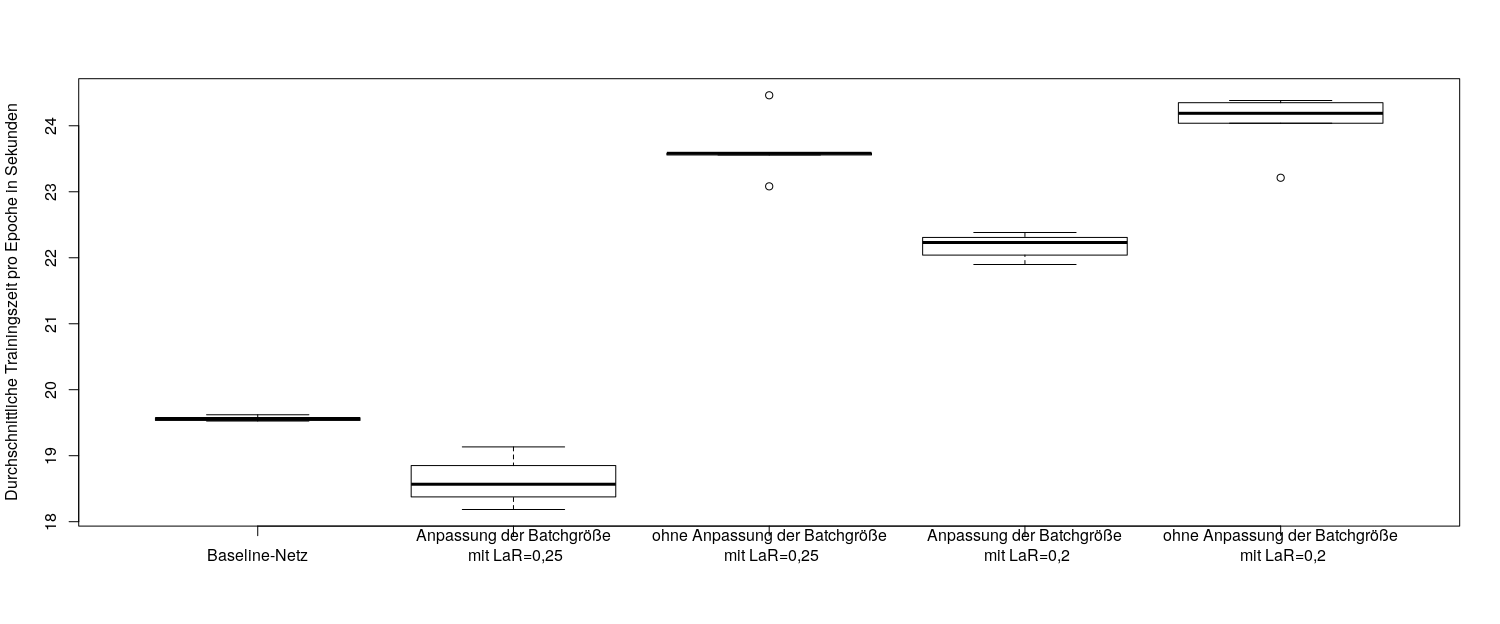
\includegraphics[width= .75\textwidth]{KapitelPartB/Images/bSize1.png}\label{abb:bSize1}}
     \hfill
     \subfloat[][]{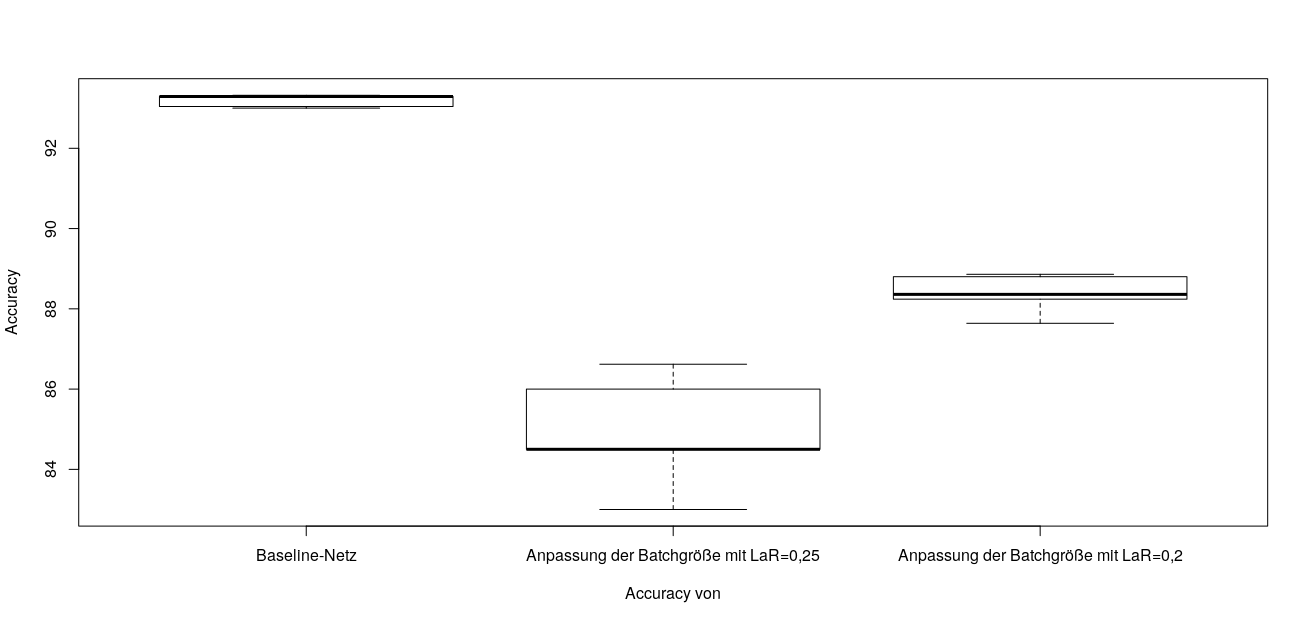
\includegraphics[width= .75\textwidth]{KapitelPartB/Images/bSize2.png}\label{abb:bSize2}}\\
     \caption{Vergleich von (a) Durchschnittlicher Trainingszeit (b) Accuracys von PruneTrain mit Anpassung der Batchgrößeund Baseline-Netz}
     \label{abb:bSize}
\end{figure}

In Abbildung \ref{abb:bSize2} ist zu sehen, wie gross der Accuracy-Verlust für das PruneTrain-Netz mit Anpassung der Batchgröße ist. Für PruneTrain mit einer Lasso-Ratio von 0,2 ergibt sich ein Accuracy Verlust von durchschnittlich 4,18 \%. Für eine höhere Lasso-Ratio ergibt sich ein Accuracy-Verlust von 7,24 \%. Diese Verluste sind wahrscheinlich auf eine nicht passende Anpassung der Lernrate in Abhängigkeit von der Änderung der Batchgröße zurückzuführen oder einer weniger häufigen Anpassung der Gewichte. Lernrate und Batchgröße hängen durch die ANzahl an Anpassungen der Gewichte zusammen: Steigt die Batchgröße, so werden weniger Durchläufe und damit weniger Gewichtsanpassungen durchgeführt. Um den geringeren zurück gelegten Weg in Richtung eines Minimum zu kopmensieren kann die Lernrate erhöht werden.














\chapter{Evaluierung von Net2Net}\label{sec:net2netexperimente}
Die Operatoren zur Beschleunigung des Lernens durch Wissenstransfer werden in diesem Kapitel evaluiert. Diese Evaluierung arbeitet mit einer selbst erstellten Implementierung auf Grundlage der Veröffentlichung zum Thema Net2Net \cite{net2net}.

Die Evaluierung umfasst drei unterschiedliche Situationen, diese Situation sind ähnlich, wie in der dazugehörigen Quelle \cite{net2net}. Die Evaluierung arbeitet mit einem ResNet, wie in Kapitel \ref{sec:baseline}. In der Veröffentlichung wird mit einem Inception Net gearbeitet. Das Inception Netz wird in Kapitel \ref{sec:inception} vorgestellt.

In der ersten Situation wird der Operator für ein breiteres Netz verwendet, um ein schmalleres Baseline Netz zu trainieren. 
In der zweiten Situation wird der Operator für ein tieferes Netz benutzt um zusätzliche Blöcke hinzuzufügen oder bestehenden Blöcken Schichten hinzuzufügen. In der dritten Situation werden beide Operatoren kombiniert. Mit der Kombination wird der Raum der möglichen Peratoranwendungen erkundet, ausgehend von einem Modell.
Die drei Situationen werden in den drei folgenden Unterkapiteln näher beschrieben. Anpassungen der Lernrate werden erst in der dritten Situation vorgenommen.

\section{Evaluierung des Operators für ein breiteres Netz}
Evaluiert wird der Operator durch verschiedene Optionen, welcher Bereich des Netzes breiter gemacht wird:
\begin{itemize}
 \item Alle Phasen
 \item Eine ganze Phase
\end{itemize}
Wie in Kapitel \ref{sec:net2net} beschrieben werden beim Operator für ein breiteres Netz die Gewichte für die neu hinzugefügten Gewichte aus den ursprünglichen Gewichten ausgewählt und so normalisiert, dass die approximierte Funktion nach Anwendung des Operators nicht signifikant von der approximierten Funktion mit den neuen Gewichten abweicht. Um zu evaluieren wie gut diese Methode funktioniert wird sie auf das schmalle Baseline Netz angewendet und verglichen mit dem schmallen und breiten Baseline-Netz. Um die Methode der Initialisierung der zusätzlichen Kanäle zu evaluieren wird als Vergleich ein Netz trainiert, bei welchem die zusätzlichen Gewichte zufällig initialisiert werden.
\begin{figure}
     \centering
     \subfloat[][]{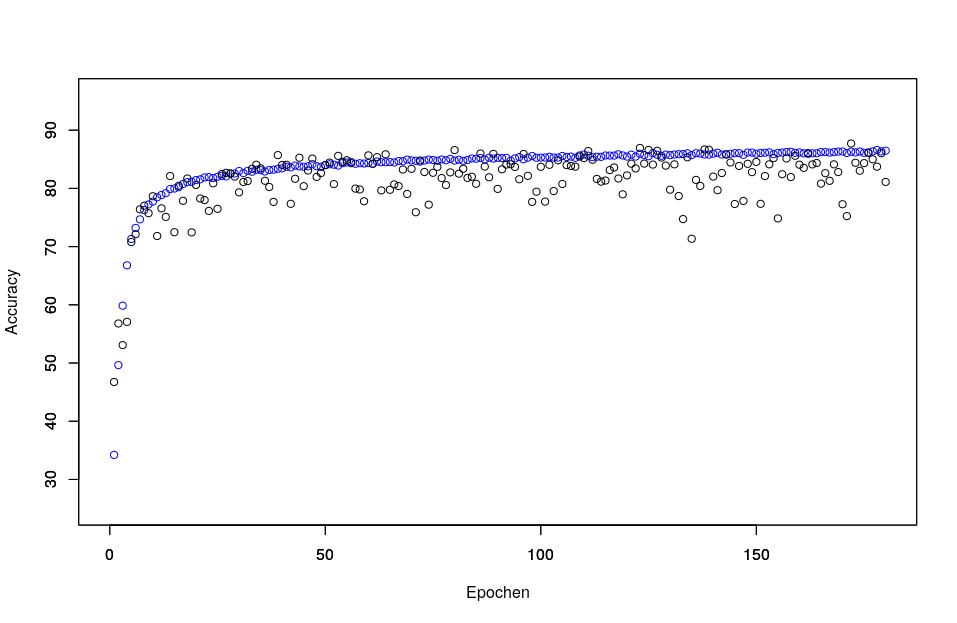
\includegraphics[width= .47\textwidth]{KapitelPartB/Images/wider1.png}\label{abb:wider1}}     
     \subfloat[][]{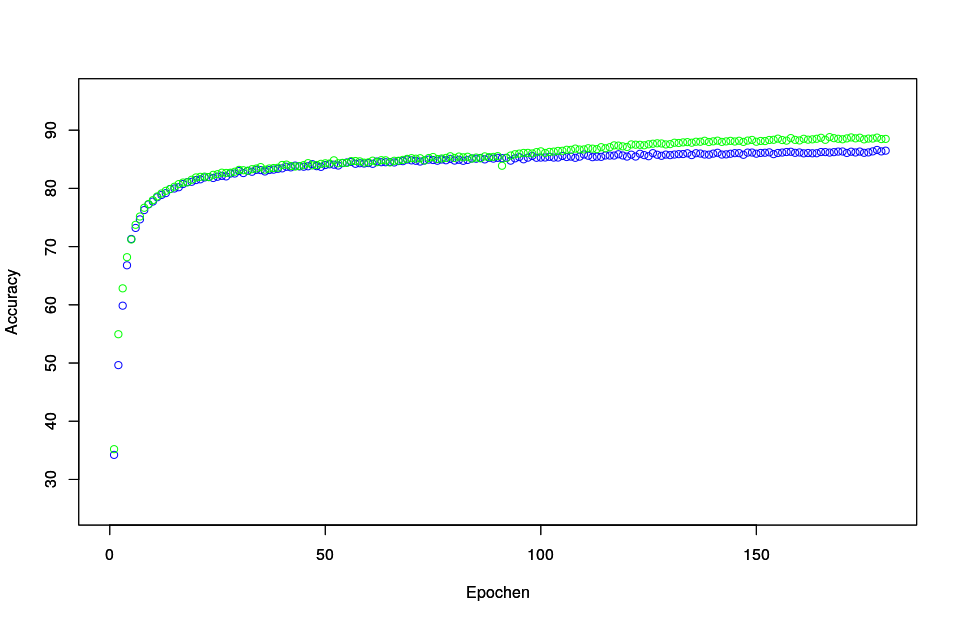
\includegraphics[width= .47\textwidth]{KapitelPartB/Images/wider2.png}\label{abb:wider2}}
     \hfill
     \subfloat[][]{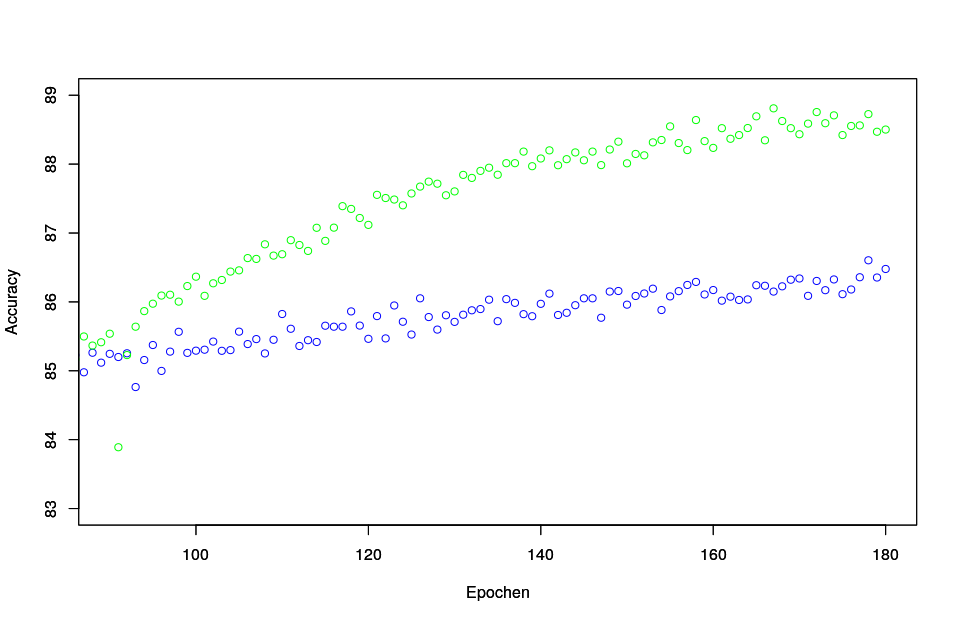
\includegraphics[width= .47\textwidth]{KapitelPartB/Images/wider3.png}\label{abb:wider3}}
     
     \caption{}
     \label{abb:memory}
\end{figure}

In Abbildung \ref{abb:wider1} ist der Verlauf der Accuracy des schmallen Baseline Netzes in blau und des breiten Baseline Netzes in schwarz über 180 Epochen ohne Anpassung der Lernrate zu sehen. Es fällt auf, dass das schmalle Baseline Netz währenddem Training wesentlich stabiler trainiert als das breite. Allerdings ist das schmalle Baseline-Netz nach wenigen Epochen bereits so weit, dass es kaum Verbesserungen gibt. Auf das schmalle Baseline Netz wird im nächsten Schritt der Operator für ein breiteres Netz angewendet. In Abbildung \ref{abb:wider2} ist der Verlauf der Accuracy des schmallen Baseline Netzes in blau im Vergleich zum schmallen Baseline Netz mit Anwendung des Operators in grün zu sehen. In Abbildung \ref{abb:wider3} ist ein Ausschnitt von Abbildung \ref{abb:wider2} für die Epochen 90 -180 zu sehen. An den beiden Grafiken ist eindeutig abzulesen, dass der Operator für ein breiteres Netz auf dem Baseline Netz die Accuracy verbessert. Die Verbesserung liegt bei den verglichenen Durchläufen bei 2 \%. 



\begin{figure}
     \centering
     \subfloat[][]{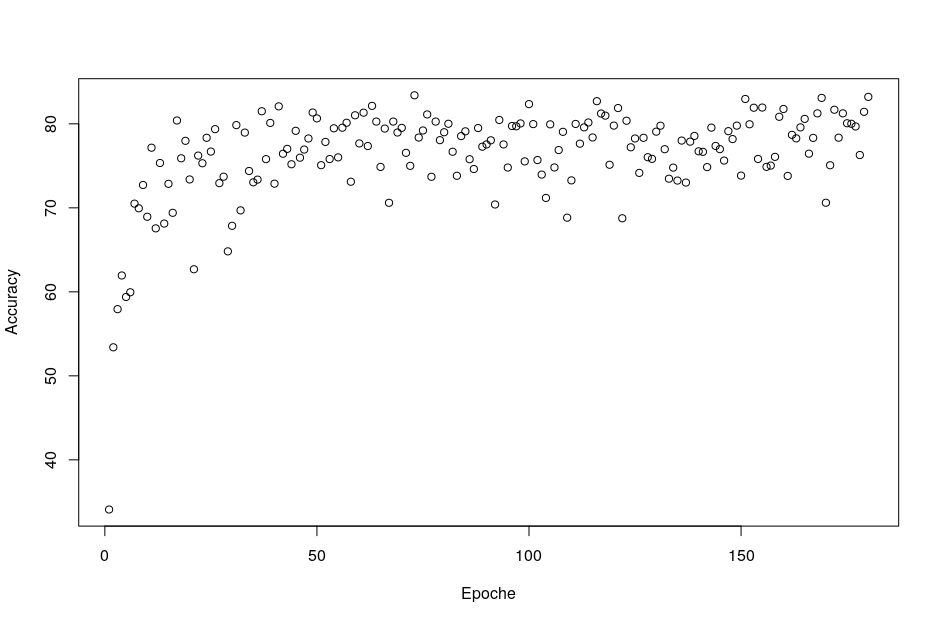
\includegraphics[width= .47\textwidth]{KapitelPartB/Images/deeperD1.png}\label{abb:deeper2}}
     \hfill
     \subfloat[][]{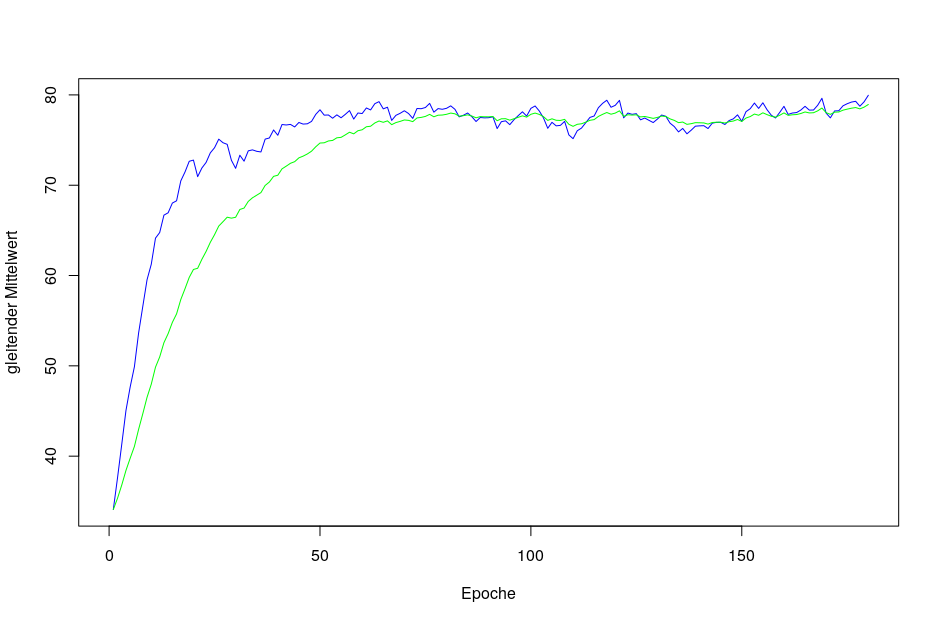
\includegraphics[width= .47\textwidth]{KapitelPartB/Images/deeperD2.png}\label{abb:deeper2}}\\
     \caption{}
     \label{abb:memory}
\end{figure}
Im nächsten Schritt muss anhand eines Entscheidungskriteriums 


\color{black}
\subsection{Verbreitern aller Phasen}
Mit Hilfe verschiedener Trainingsprotokolle wird untersucht, wie der Operator für ein breiteres Netz die Klassifikationsleistung des Netzes verändert.
Zunächst wird überprüft, welches Ergebnis bei Anwendung des Operators für ein breiteres Netz auf das schmalle Baseline-Netz nach 180 Epochen Training herauskommt. Nachdem Anwenden des Operators wird mit dem gleichen Trainingsprotokoll für weitere 180 Epochen trainiert. In Abbildung \ref{abb:allN2N1} ist abgebildet, wie der Verlauf der Accuracy für Net2Net mit zwei verschiedenen Möglichkeiten, die neuen Gewichte zu initialisieren, ist. In Blau dargstellt wird der Verlauf der Accuracy für die zufällige Initialisierung der neuen Gewichte durch das Verbreitern des Netzes.
Es ergibt sich, wie in der größeren Abbildung \ref{abb:allN2N2} zu sehen ist eine minimale Verschlechterung durch das Anwenden des Operator für ein breiteres Netz im Vergleich zum Baseline-Netz.
 \begin{figure}
     \centering
     \subfloat[][]{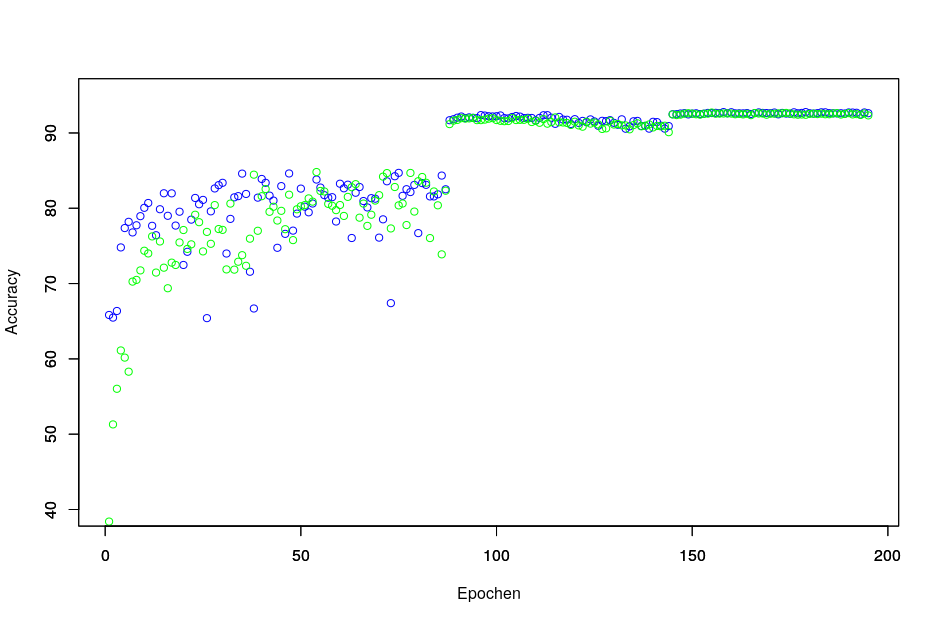
\includegraphics[width= .47\textwidth]{KapitelPartB/Images/n2nWiderAll1.png}\label{abb:allN2N1}}
     \hfill
     \subfloat[][]{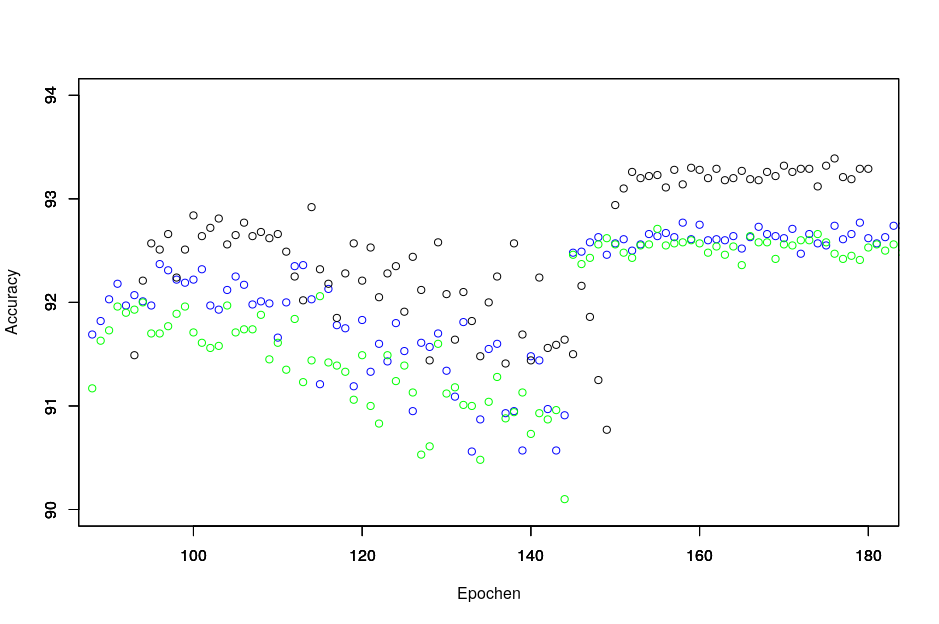
\includegraphics[width= .47\textwidth]{KapitelPartB/Images/n2nWiderAll2.png}\label{abb:allN2N2}}\\
     \caption{Vergleich der Accuracy bei verschiedenen Initialisierungsmöglichkeiten des Operators für ein breiteres mit dem Baseline Netz: (a) alle Epochen (b) Zoom auf die Epochen 90 bis 180. Blau zeigt die Accuracy der Initialisierung der zusätzlichen Gewichte mit zufälligen Werten. Grün zeigt die Initialisierung mit den Werten aus dem restlichen Tensor. Schwarz zeigt das Baseline-Netz als Vergleich.}
     \label{abb:memory}
\end{figure}
Um den Operator für ein breiteres Netz besser verwenden zu können wird im nächsten Schritt übrprüft, ob mit einer häufigeren schrittweisen Anpassung der Lernrate und mit weniger trainierten Epochen nach Anwenden des Operator ein besseres Ergebnis möglich ist.


\section{Evaluierung des Operators für ein tieferes Netz}
Zur Evaluierung des breiteren Netzes wird zunächst wie in der Veröffentlichung jeder Block um eine Schicht erweitert. Dabei werden die zusätzlichen Schichten wie in Kapitel \ref{sec:deep} beschrieben initialisiert. Als Vergleich dient das Baseline-Netz aus Kapitel \ref{sec:baseline}.

\todo{Ergebnisse}

Eine weitere Verwendung des Operators für ein tieferes Netz ist die Möglichkeit einen neuen Block hinzuzufügen. Nur ein einfaches Hinzufügen würde hier zu Problemen führen. Der Grund hierfür ist Abbildung \ref{abb:deeper} dargstellt. Dabei soll an einer Verbidung, die bisher die Daten von einer Schicht zur nächsten transportiert ein neuer Block inklusive Kurzschlussverbindung entstehen. Der hinzuzfügende Block blau \todo{blau markieren} markiert. Der neue Block soll wie die Kurzschlussverbindung die Identität berechnen. Betrachtet $x$ als Größe der Identität. Dann wird hier mit dem neuen Block staat $x$ das doppelte, also $``X$ berechnet. Um dieses Problem zu umgehen wird an jeder Additionsstelle für eine Kurzschlussverbindung eine Multiplikation mit 0,5 berechnet (rechte Seite der Grafik). So wird nicht mehr $x$ sondern $0,5x +0,5x=x$ berechnet.

Zunächst wird dieses Netz trainiert ohne einen Operator anzuwenden. In Abbildung \ref{abb:BaselineMul1} ist ein Boxplot abgebildet, der die Accuracy des Netzes mit zusätzlichen multiplikativen Faktoren mit dem Baseline-Netz vergleicht.

 \begin{figure}
     \centering
     \subfloat[][]{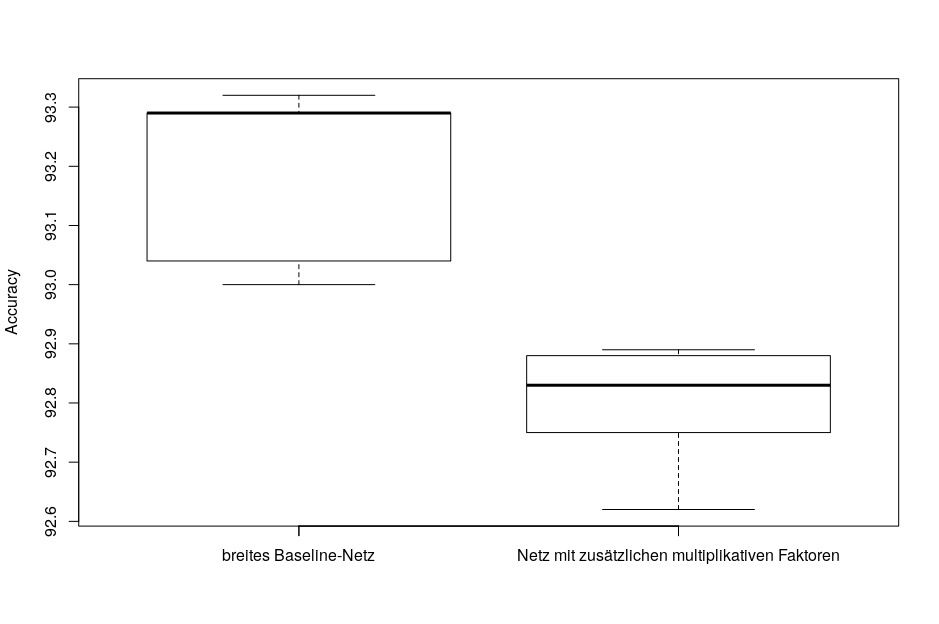
\includegraphics[width= .75\textwidth]{KapitelPartB/Images/baselineMul1.png}\label{abb:BaselineMul1}}
     \hfill
     \caption{Vergleich von }
     \label{abb:BaselineMul}
\end{figure}


\begin{figure}[h]
 \centering
 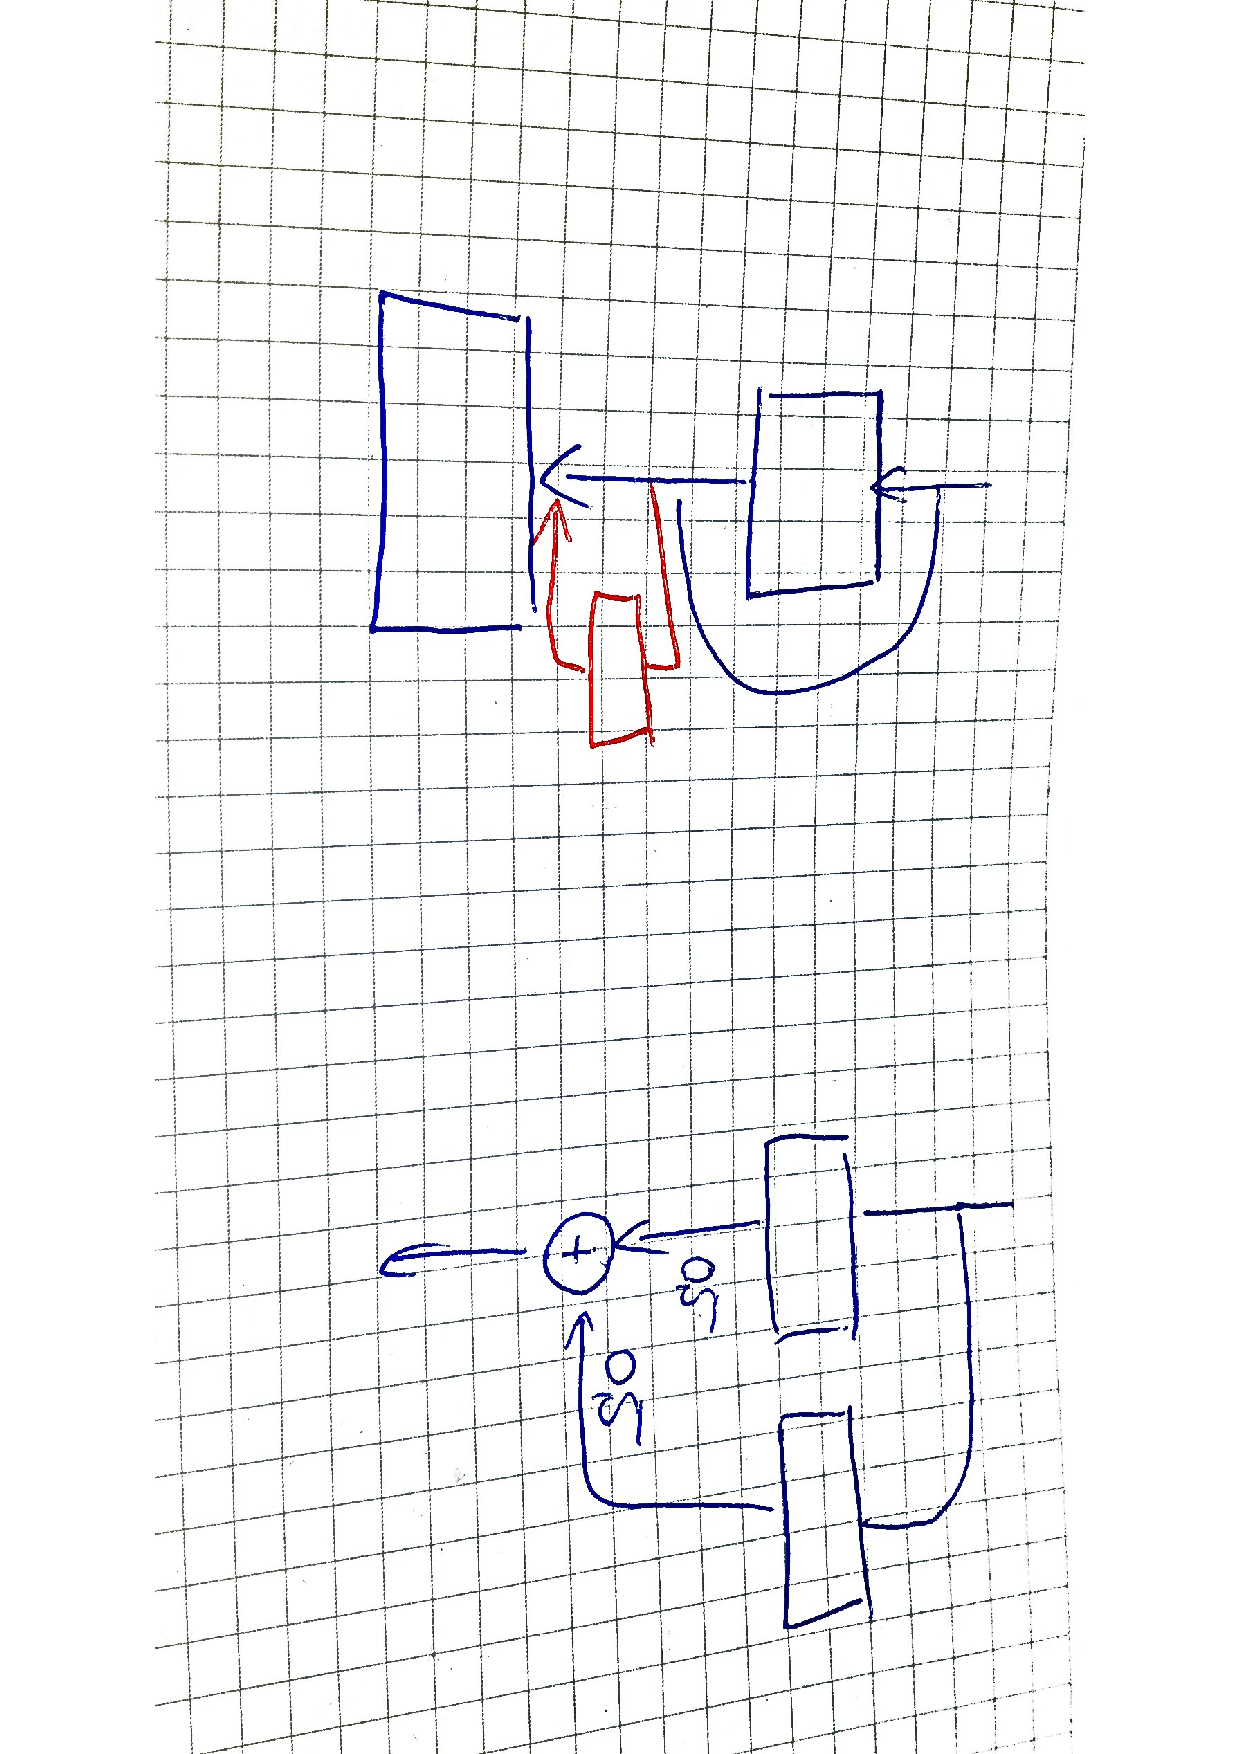
\includegraphics[width=0.5\textwidth, angle=90]{KapitelPartB/Images/deeper.pdf}
 % deeper.pdf: 0x0 px, 300dpi, 0.00x0.00 cm, bb=
 \label{abb:deeper}
\end{figure}




\section{Erkunden des Modellraums}

 \begin{figure}
     \centering
     \subfloat[][]{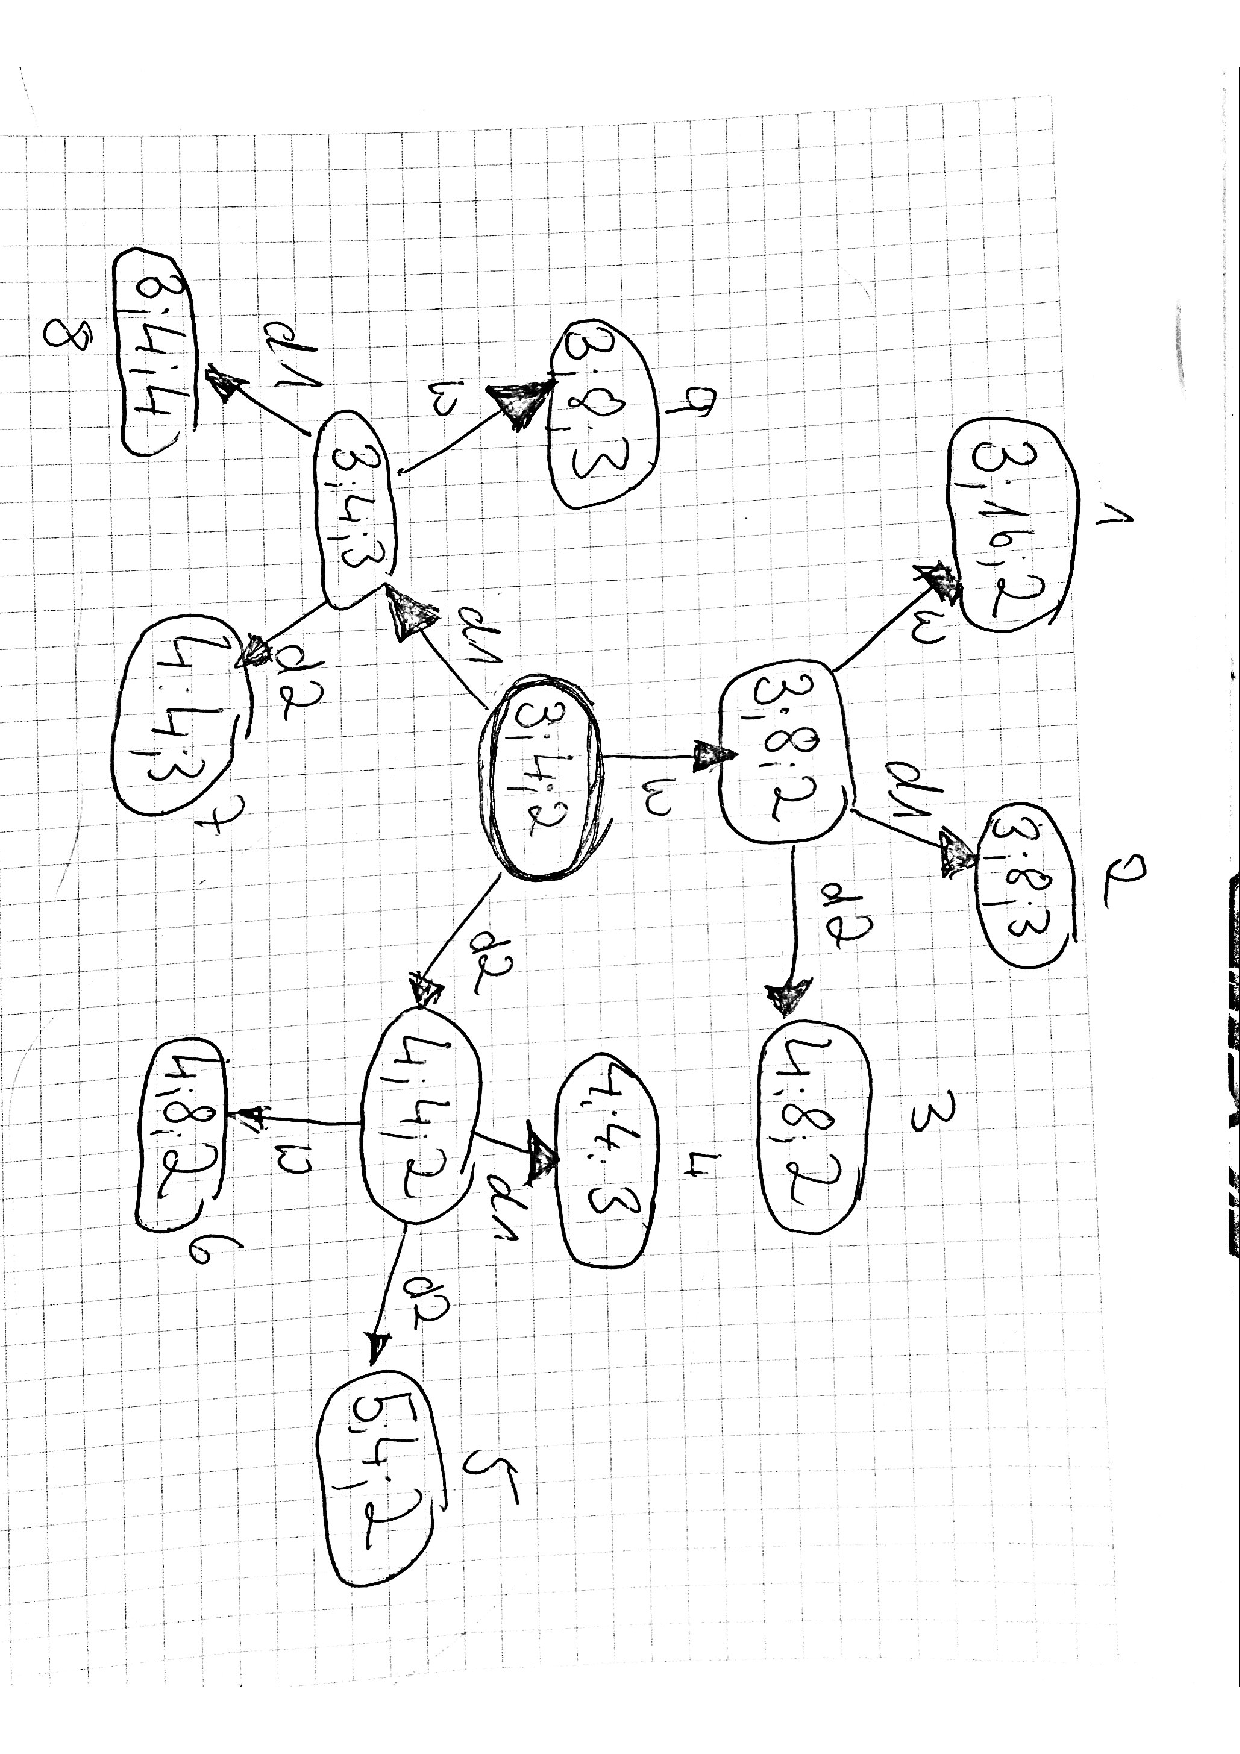
\includegraphics[width= .75\textwidth, angle=90]{KapitelPartB/Images/deeperRoom.pdf}
     \label{abb:deeperRoom1}}
     \caption{Anzahl an Blöcken pro Phase; Breite der ersten Schicht; Schichten pro Block}
     \hfill
\end{figure}




\chapter{Ausblick und Fazit}\label{sec:fazit}
Es hat sich gezeigt, dass MorphNet den Nachteil hat, dass die Tiefe des Netzes nicht verändert werden kann. Diesen Nachteil kann Net2Net als potentieller Kandidat einer erweiternden Methode einer Kombination ausgleichen. Es zeigt sich bei allen Verfahren, dass eine Anpassung der Lernrate Sinn macht. 

Es wäre sowohl für MorphNet als auch für die Kombination ein potentieller Gewinn, wenn die Lernrate automatisch angepasst werden würde, bevor eine Anpassung der Struktur passiert. Der Grund, wieso dies sinnvoll ist liegt daran, dass ohne Anpassung der Lernrate nicht das volle Potential jedes Modells genutzt werden kann. Hier wäre es allerdings notwendig nach der Veränderung der Struktur zu evaluieren, wie mit der Lernrate weiter zu verfahren ist. Die Anpassung der Lernrate sollte hier sowohl bei einem Plateau in der Accuracy als auch bei nicht stabilen Training funktionieren.


Da sich beim Training der verschiedenen Netze gezeigt hat, dass diese unterschiedlich lange brauchen, um ihr Potential auszuschöpfen ist es sinnvoll die Epoche zu der ein Operator von Net2Net angewendet wird flexibel anhand des Accuracy Verlaufs zu gestalten.  


Die Erkundung des Modellraumes zeigt, dass sich Net2Net auch bei kleinen Ausgangsnetzen lohnt. Für die Kombination wäre es hilfreich, mit Hilfe der Ergebnisse des Beschneidens zu entscheiden welcher Operator angewendet wird. 

Bei den verschiedenen Verfahren ist zu beobachten, dass in allen vorgestellten Fällen ein Trade-off zwischen Accuracy und Trainingszeit zu beobachten ist.


% Anhang ---------------------------------------------------------------
%
\cleardoublepage
\appendix

%========================================================================================
% TU Dortmund, Computer Science VII
%========================================================================================
\chapter{d}


%
\listoffigures
\addcontentsline{toc}{chapter}{Abbildungsverzeichnis}
\cleardoublepage


\cleardoublepage

%
\addcontentsline{toc}{chapter}{Literaturverzeichnis}
\bibliographystyle{alpha}
\bibliography{Literature}

% ----------------------------------------------------------------------

\end{document}
